\newchapt{The New Enhancement}{chapt10}{The New Enhancement}

%% \section{Major Plane Detection}
%% Given a point cloud dataset of a building, its major planes can be detected using plane based hough
%% transform method. Once the major planes are identified, we can rectify the dataset and project the
%% 3D data into 2D slices along the normals of those major planes.
%%
%% *. Major planeqs detection.
%%
%% *. Data Rectification.

\section{New Improvement Overview}

With the windows detection and segmentation improvement, the overview of the new enhancement is depicted 
in the \Fig{model_ov}. If there is no window or door detected at the window/door detection module, 
the window/door installation module would be skipped.

\begin{figure}[htbp]
  \centering
  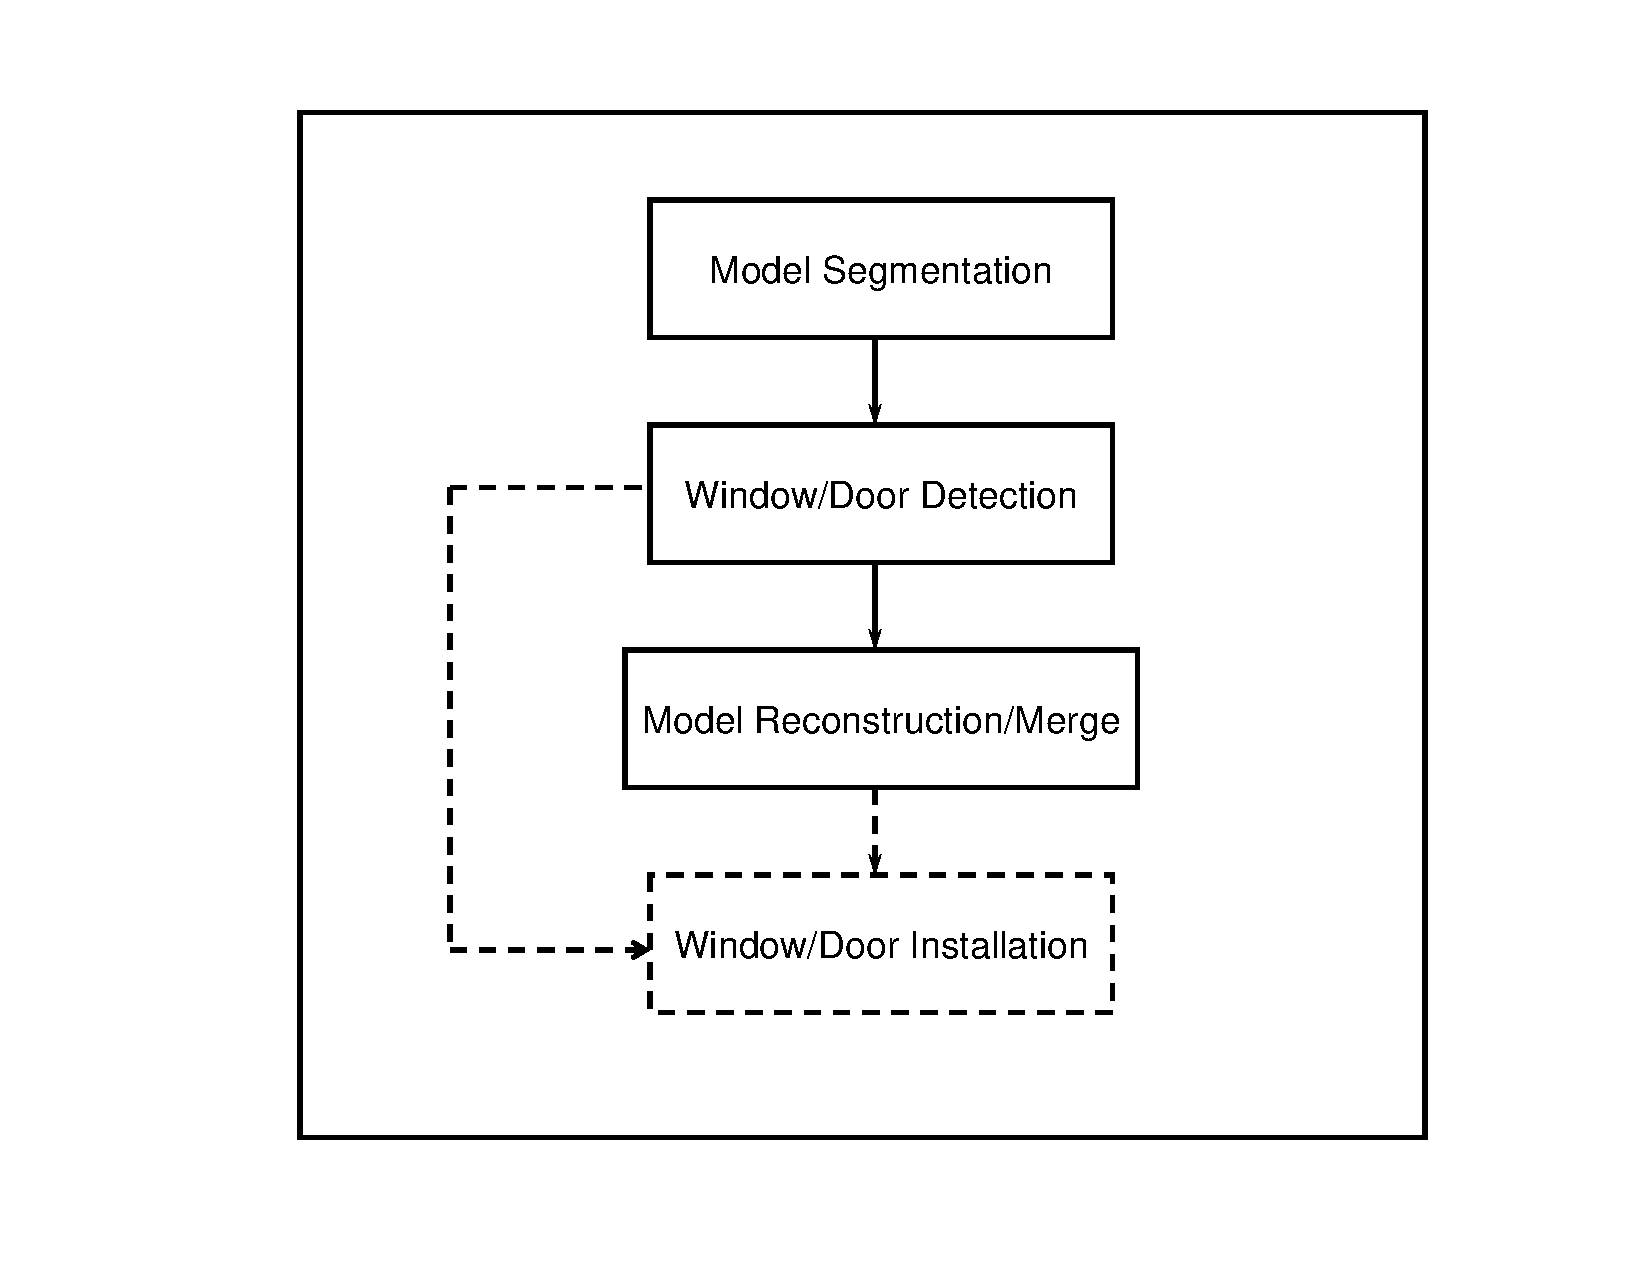
\includegraphics
      [width=\textwidth]
      {model_overview.pdf}
      \caption{The flow diagram of the new enhancement.}
      \label{fig:model_ov}
\end{figure}


\section{Model Segmentation}

%% The main functionality of buildings is to provide a space for people to live or work.
%% Therefore, the main structure of them can be as simple as a box with windows.
%% On the other hand, buildings are the results of architectures, which can be considered as art.
%% This could make the structures of buildings extremely complicated.

Modeling a building as a whole structure from point cloud is complicated 
due to the natural complexity of buildings.
To tackle this issue, buildings should be split into simpler sub-structures for reconstruction.
We can utilize this divide and conquer strategy to segment the point cloud dataset of a building
and reconstruct each segmented dataset based on extrusion or tapered operations.
Once each segmentation is processed and modeled, they can be combined and merged into the whole final model.

%% (OPTION) We proposed a multi-resolution segmentation approach, that is separator based and keyslice based
%% segmentation. The idea is to first decompose the whole building using separator slices detected from
%% all major facades. This segmentation step is relative safe and precise in a sense that
%% the separators or salient planar feature generally separate parts from each other.
%% The segmentation consists of two steps; the first one is separate the data based on separators detected
%% in slices from all major directions. We shall obtain split data after the first step.
%% The second step is to further segment these split data if necessary.

As we know, different parts of a building are separated by walls, ledgers etc. 
These {\it ``separators''} provide clues for model segmentation. 
When projected onto 2D images, these separators have a common characteristic, 
that is a relative large {\it ``dark''} region representing a salient feature in black-white images.
For example, the roof and the body are divided by a ledger as shown in \Figc{MS_Fig1}.
\Figb{MS_Fig1} and \Figd{MS_Fig1} shows different parts of the roof are separated by walls.


\begin{figure}[htbp]
  \centering
  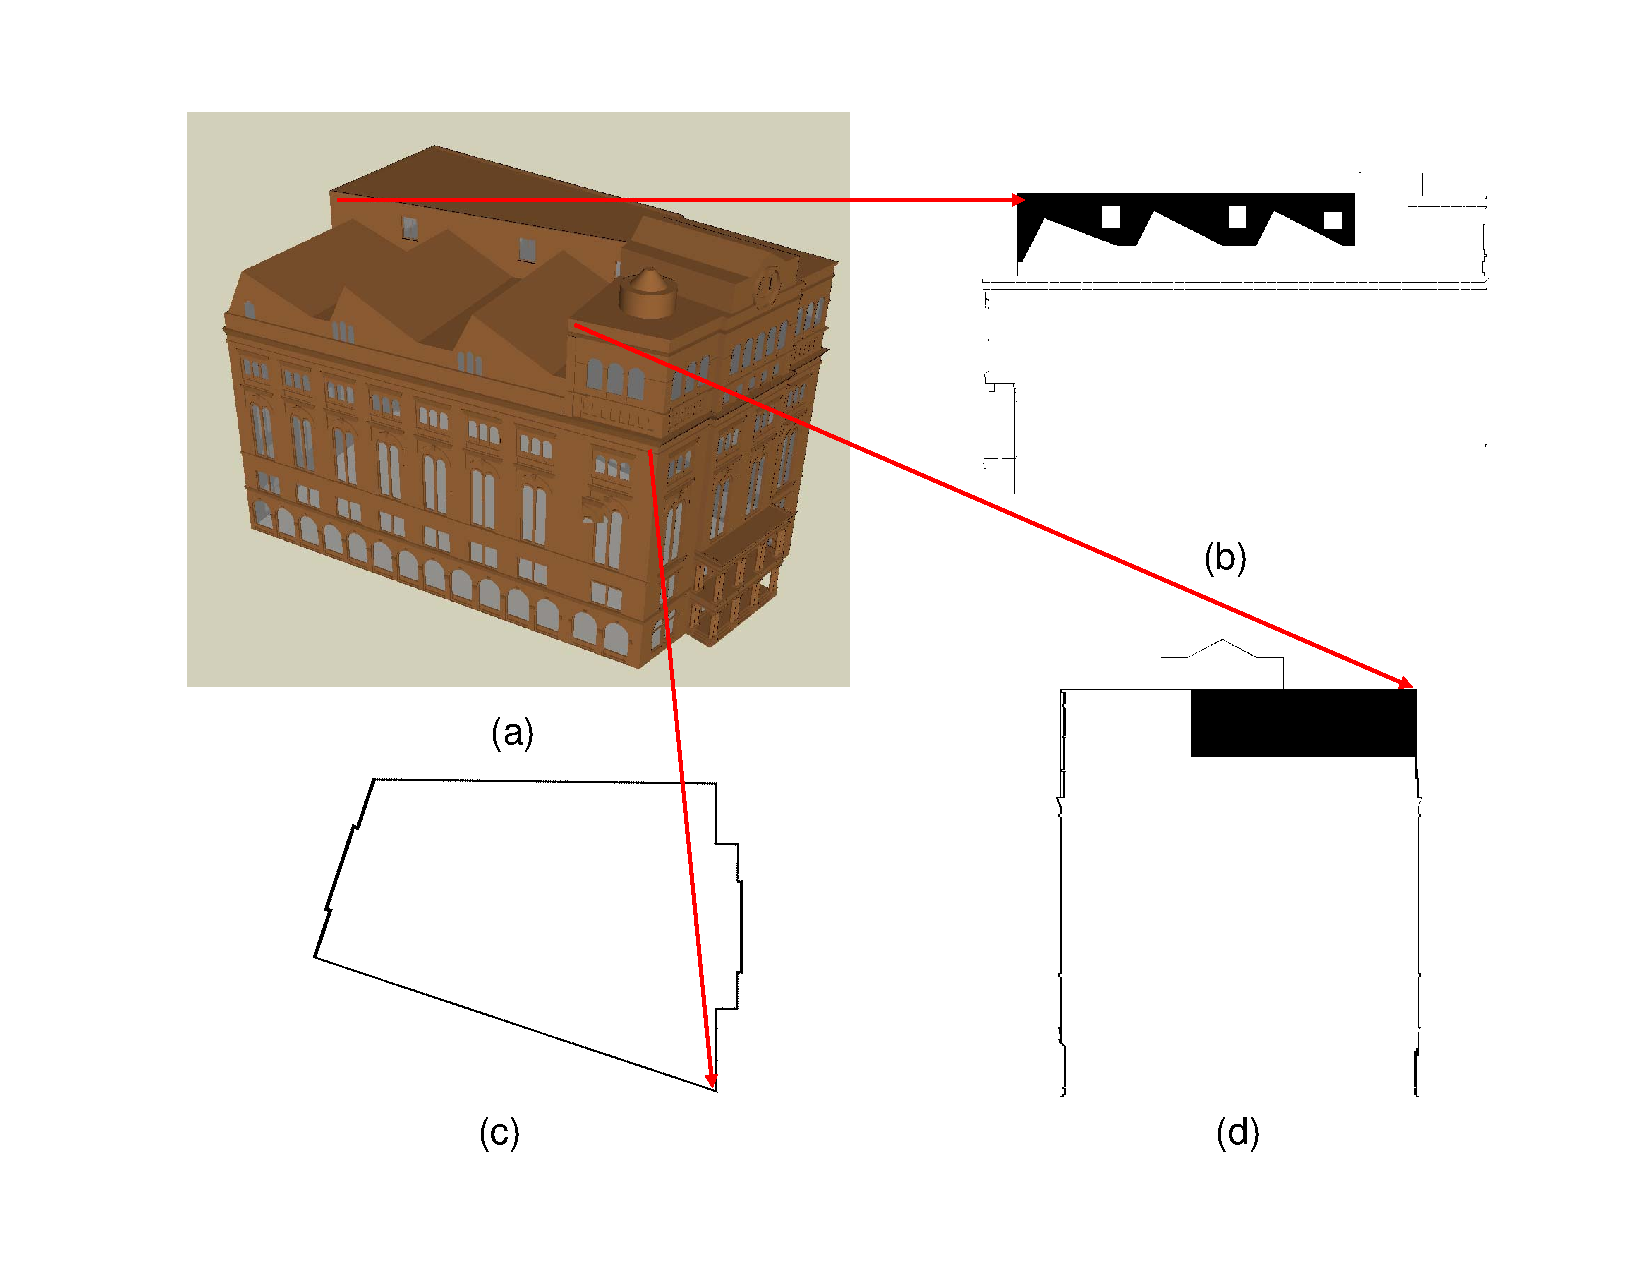
\includegraphics
      [width=\textwidth]
      {model_separate.pdf}
      \caption{The model segmentation: 
      (a) the original cooper union model.
      (b) the projected wall image from one face.
      (c) the projected wall image from another face.
      (d) the projected ledger image.}
      \label{fig:MS_Fig1}
\end{figure}

The model segmentation is carried out as follows:
First of all, for a given point cloud dataset, we'll compute separators from all major directions, 
including bottom-up and normals of facades. 
Because a building may have multiple facades with normals perpendicular to the bottom-up direction,
it is much easier to segment dataset in bottom-up direction if there is any separators detected.
The next step is to compute the segmentation image from the separators of those normals.
Finally, we segment the remaining dataset based on the segmentation image.

\subsection{Separator Detection}
\label{sec:sd}

We used a kernel based connected components (CC) method for separator detection. 
For each projected slice image $I_i$, the separator detector 
checks each data point $P_i$ using a 5x5 kernel $K$ centered at $P_i$.
Let $S_p$ be a set of points visited by the separator detector and $S_p$
is initialized to empty.
At the beginning, the point $P_i$ is checked against $S_p$ to 
determine whether it has been visited before. 
If not, $P_i$ is added into $S_p$ and the data points $N={P_j | P_j \neq P_i, P_j \in K}$ 
covered by $K$ are recorded.
If there are enough data points found in the neighbor, say $|N| > 12$, 
namely half of the kernel $K$, 
$P_i$ is considered as qualified point for a new connected component $C$.
For this case, $P_i$ is added to $C$. 
The same computation is applied to all new recorded data point in $N$, and 
qualified points are added into $C$. 
When there is no more new data point needs to be checked, the detector stops
and a new connected component, $C$, is detected.


The minimum and maximum coordinates, $x_{min}, x_{max}, y_{min}, y_{max}$, in $C$
are computed to obtain the rectangle boundary. 
To check whether $C$ represents a real separator, a testing is carried out:
\begin{equation*}
\left\{
\begin{array}{lr}
| x_{max} - x_{min} | > T_{size} \\
| y_{max} - y_{min} | > T_{size}
\end{array} \right.
\end{equation*}
where $T_{size}$ is a threshold representing the minimum size of the separator, 
usually a value of 16 is good enough to rule out all non-separators.
The above testing implies that a real separator CC should contains a big chunk of data
and its width and height should be at least $T_{size}$. 
If a connected component $C$ satisfies the above conditions, 
the slice index $i$ and the bounding information $x_{min}, x_{max}, y_{min}, y_{max}$, 
are logged down for further process.

\subsection{Dataset Segmentation}

The separators in all major directions computed in the previous section will be used for model segmentation.
If there are separators detected in bottom-up direction, the first step is to segment the dataset based on 
these separators. Because there is only one direction, the segmentation is straightforward.
The next step is to transform the separators in all other directions into the common coordinate.
As \Figa{DS_Fig1} shows, each separator is transformed into a line segment in the bottom-up 
projected image with the end points representing the bounding positions.
To divide the dataset, we need to know the exact boundary for each segmentation. 
This can be done by computing exact intersection point for each line segment with other line segments.


\begin{figure} [htbp]
\begin{center}
\begin{tabular}{cc}
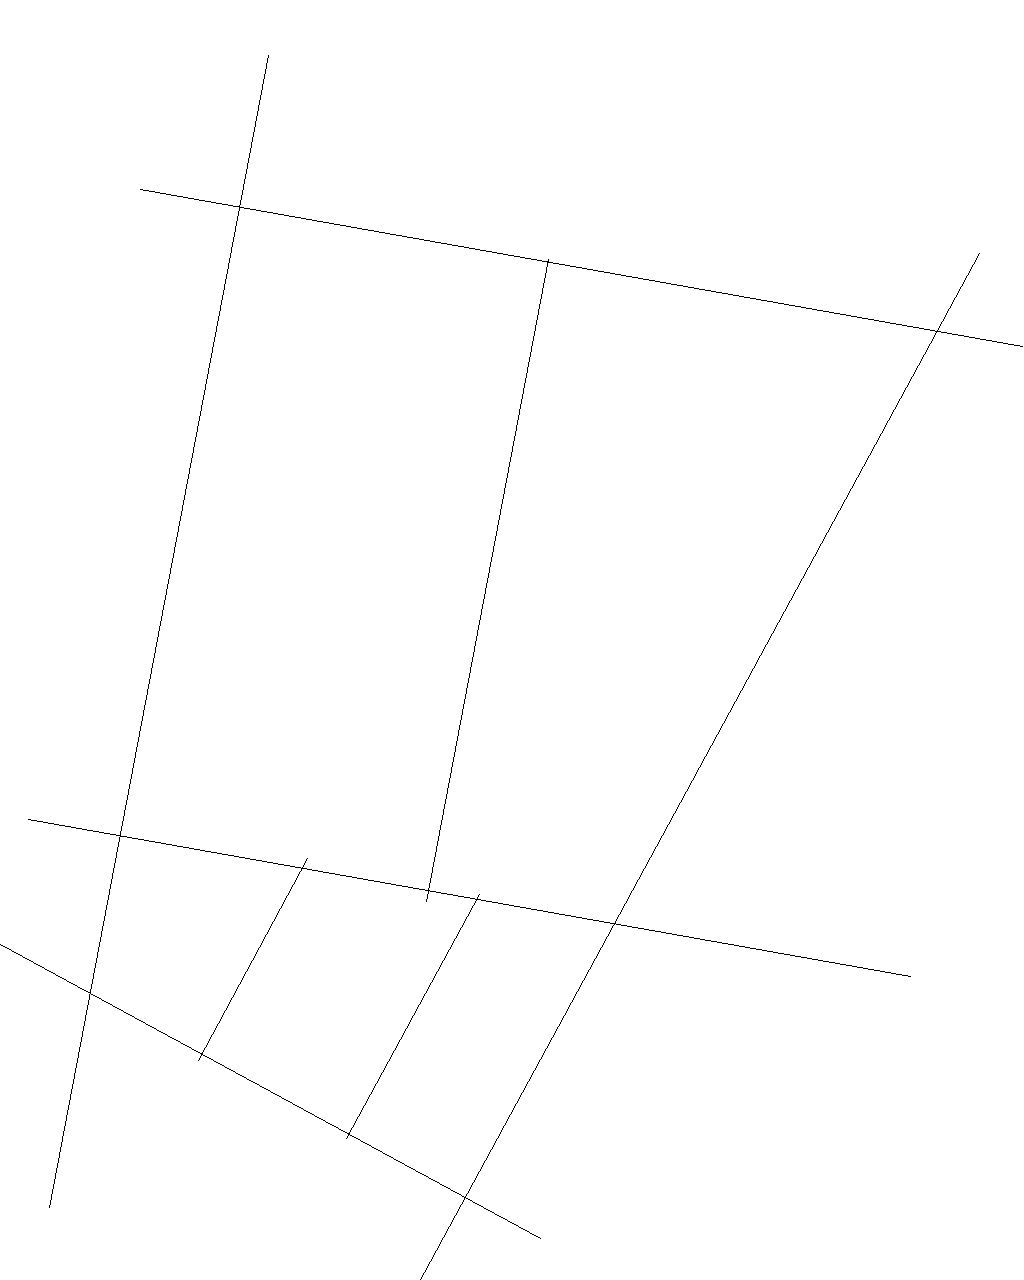
\includegraphics[width=0.5\textwidth]{segment_roof_result.png} &
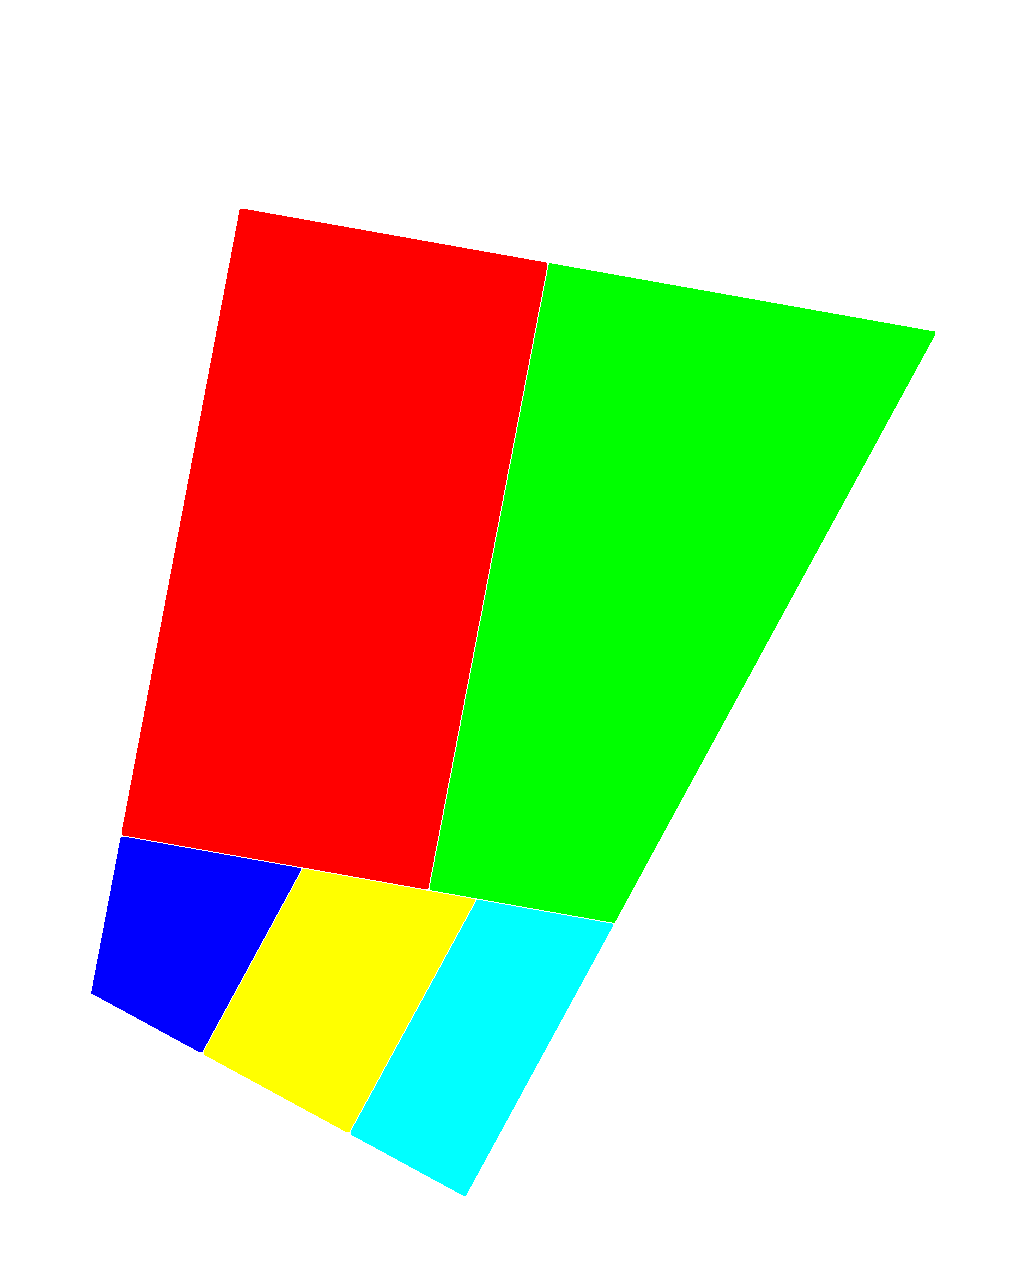
\includegraphics[width=0.5\textwidth]{segment_roof_regions.png} \\
(a) & (b) 
\end{tabular}
\end{center}
\caption{ Segmentation region computation:
      (a) the transformed image with line segment of the separators
      (b) the processed segment image}
\label{fig:DS_Fig1}
\end{figure}

Given a line segment $L_i = P_0P_1$, represented by two end points $P_0$, $P_1$, 
we can compute the intersection points of
$L_i$ with all other line segments. %[ with the equation of intersection computation of two planar lines].
If the result intersection point $P_i$ is falling outside of the image or 
is far away from either $P_0$ or $P_1$, $P_i$ can be skipped. 
When all the other line segments are checked, we can obtain two intersection points
, $P'_0$ and $P'_1$ which are the closest ones to $P_0$ or $P_1$ respectively. 
After intersection points are computed for all line segments, 
the segmentation image $I_s$ can be obtained as shown in \Figb{DS_Fig1}.

With the segmentation image $I_s$, the dataset segmentation is straightforward. 
We first build up a look-up table for each pixel in $I_s$ as shown in \Figb{DS_Fig1}. 
Different regions are marked in different colors and are assigned a unique region id $rid$. 
For any 3D point cloud data $P$, we can compute
its 2D projection location $(x, y)$ in the image $I_s$. %[ based on the equation [equation of the projection].
The region id for $P$ can be obtained from the look-up table based on $(x, y)$ coordinates.
In the example shown in \Figb{DS_Fig1}, 
totally 5 regions are identified and the original point dataset is split into 5 subsets for further process.

\section{Windows and Doors Detection}
\label{sec:wdd}

\begin{figure}[htbp]
  \centering
  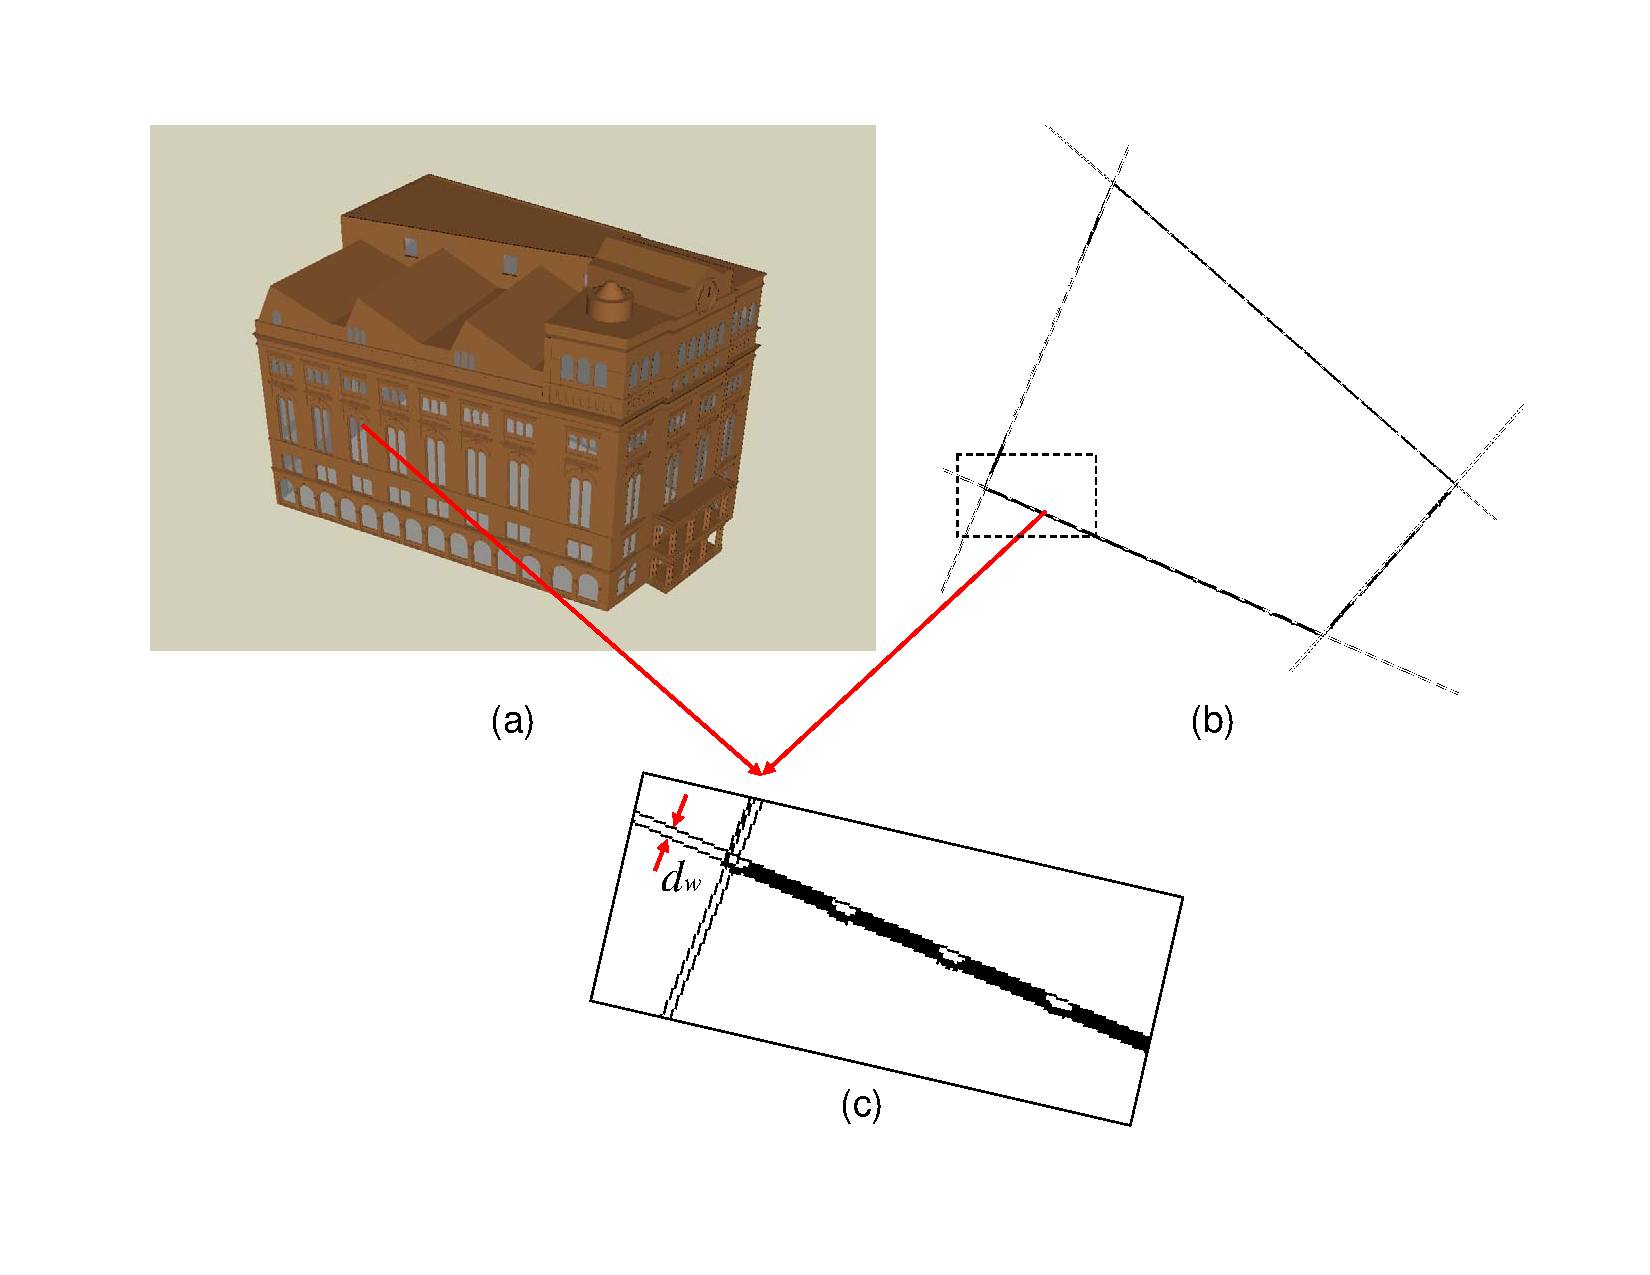
\includegraphics
      [width=\textwidth]
      {model_win_comp.pdf}
      \caption{The thickness detection of the windows/doors:
      (a) the window on the original model
      (b) the projected slice viewing from bottom-up direction
      (c) the close-up view of the parallel lines and the distance $d_w$. }
      \label{fig:WD_Fig1}
\end{figure}

Windows and doors are important features for buildings to be modeled. 
%Furthermore, accurate computation of the extrusion structures requires these information.
%Without knowing the marked location as window part, 
%extra keyslices may be computed and hence lead to unnecessary extrusion operations. 
%[show a figure with unnecessary keyslice? how?]
The information we want to compute for windows and doors includes both the location and the thickness.
The thickness is computed based on the observation that two parallel lines can be detected
when viewing from the bottom-up direction as shown in \Figc{WD_Fig1} . 
For two parallel lines $L_1: y = mx + c_1$ and $L_2: y = mx + c_2$, 
% as shown in Fig1, http://www.askiitians.com/iit_jee-Straight_Line/Distance_between_two_parallel_lines
the distance $d_w$ is computed with the following equation,
\begin{equation*}
d_w = \frac{|c_1 - c_2|}{\sqrt{1 + m^2}}
\end{equation*}

%[Fig1: show the window thickness detection image, two parallel lines are drawn]
%[Fig2: show the projected windows/doors slice]

\begin{figure}[htbp]
  \centering
  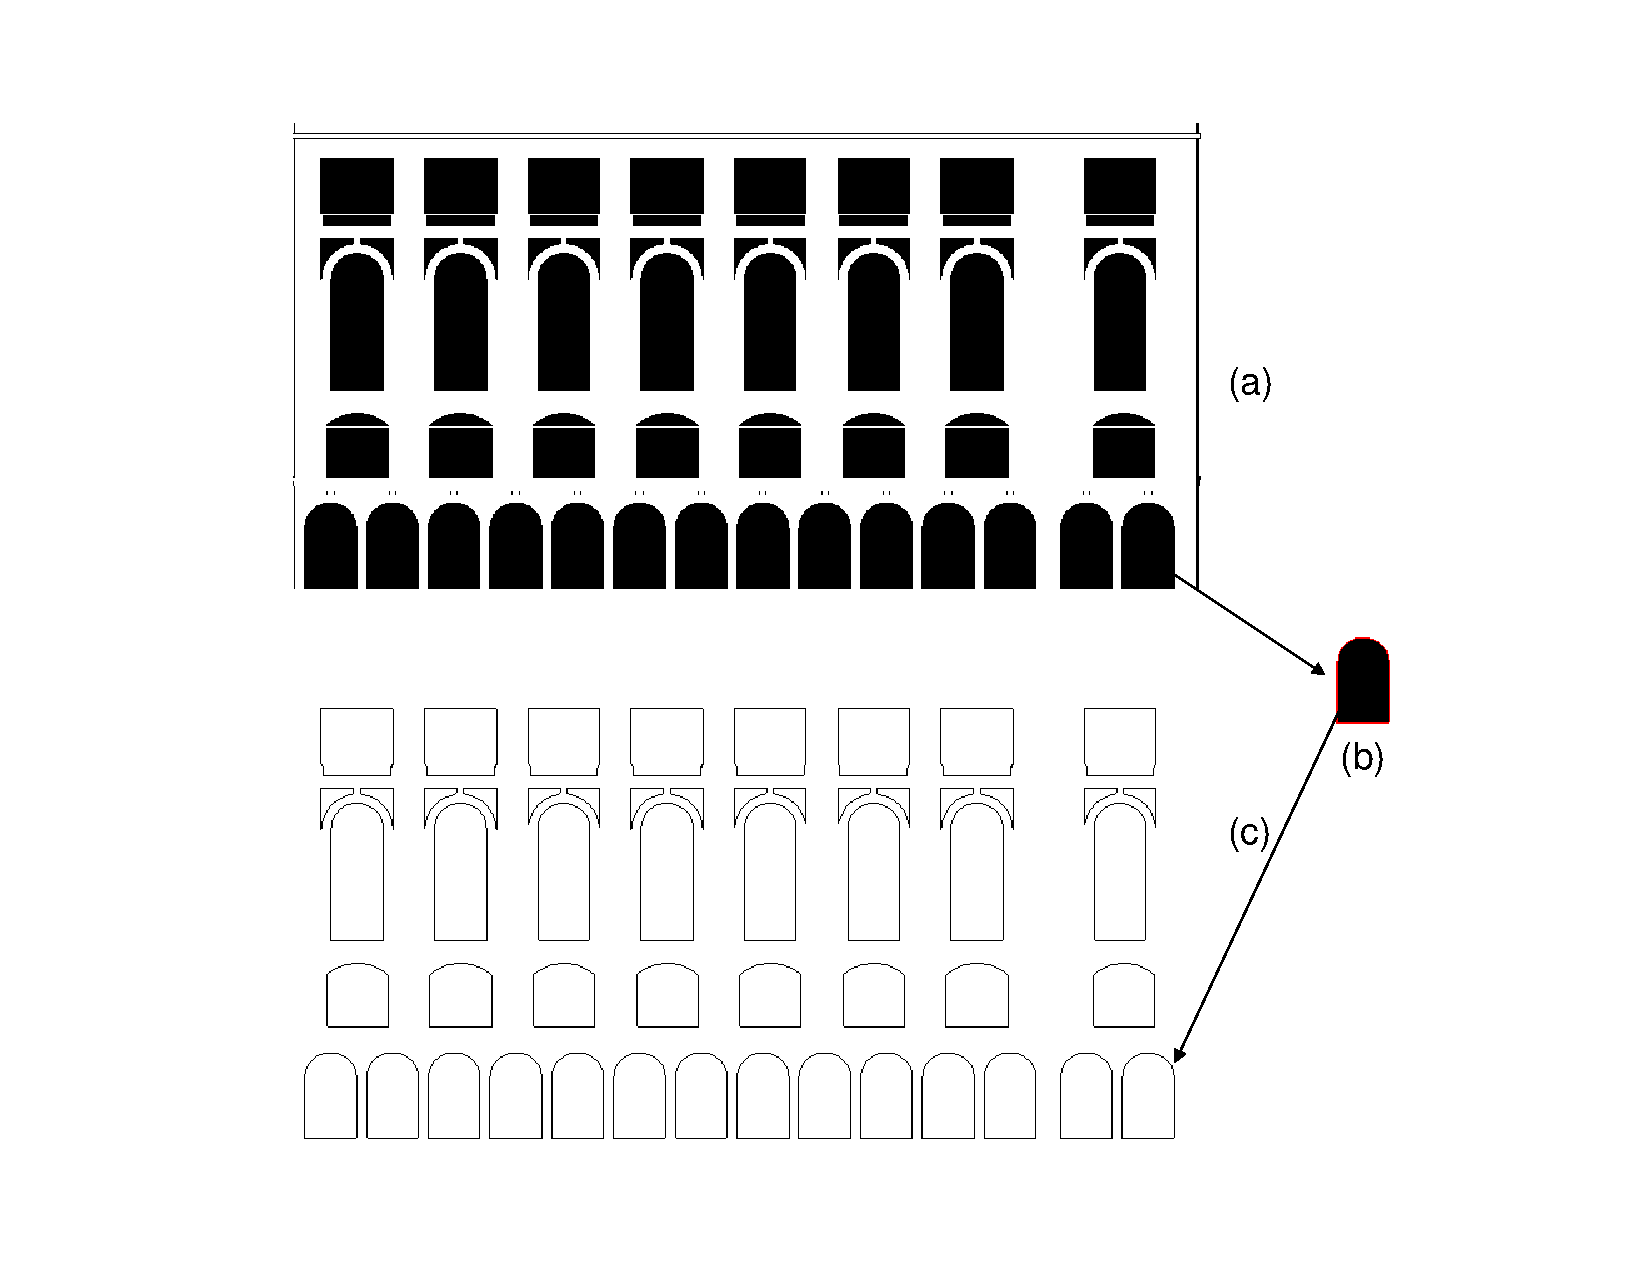
\includegraphics
      [width=\textwidth]
      {window_result.pdf}
      \caption{The window information: (a)The projected windows slice
      (b) the most bottom-right window extracted from (a) with BPA contour in red. 
	(c) The contours of windows computed from (a).}
      \label{fig:WD_Fig2}
\end{figure}

Once the distance $d_w$ is computed, we can obtain the windows/doors image by projecting the data points
between $L_1$ and $L_2$ onto a slice image as shown in \Figa{WD_Fig2}. 
There are multiple window structures in the same projected slice image. 
We can use the same strategy as separator detection described in Section \ref{sec:sd}, that is,
kernel based connected component method, to isolate each window for processing. 
\Figb{WD_Fig2} shows a window extracted as a connected component and BPA algorithm was applied
to obtain the contour in red.
After walking through the image shown in \Figa{WD_Fig2} for all the connected components 
and applying BPA on them, 
the final results show all the detected window contours as depicted in \Figc{WD_Fig2}.
These contours will be used to add windows and doors onto the final model.

%% \subsection{Windows and Doors Mask Image Generation}
%% 
%% After computing the windows and doors structures for each facade, 
%% these information can be used for accurate keyslice detection. 
%% As we mentioned before, the keyslice detection based on Hausdorff distance criteria may
%% introduce unnecessary keyslice due to the data of windows or doors. 
%% To tackle this issue, we can construct a series of windows and doors mask images 
%% from the computed structures and therefore eliminate those unnecessary keyslices.
%% 
%% With the information computed on the windows, the mask image generation is straightforward.
%% For each window, we can obtain the 3D bounding box around it based on the $d_w$ and
%% the size of the window in 2D image. The task is to convert these 3D bounding box for each
%% window to corresponding rectangle in 2D slices for each direction. 
%% Once we get this rectangle box for a direction, say $X$, we can use it as a mask when
%% computing keyslices in $X$ direction.
%% 
%% [Figaxxx] shows that 4 projected window slices and the rectangle boxes in bottom-up direction
%% for all windows in all 4 directions are shown in [Figbxxx]. 
%% Likewise, we can generate similar mask image for other directions.
%% 


\section{Model Reconstruction}

When underline structures of all segmentations have been computed, we can start to reconstruct the whole model.
The reconstruction of a single segmentation is straightforward: transform the underline geometry polygon to
3D coordinate system; for an extrusion structure, it is a push-pull operation of the basic geometry;
for a tapered structure, it is a face constructions between the base line segment and the corresponding
converging point.

The reconstruction becomes more complicated when multiple segmentations need to be merged since
some segmentations may share the same vertices or edges. Therefore model merging needs to be done
for the reconstruction of the whole model.

\subsection{Model Merging}


\begin{figure}[htbp]
  \centering
  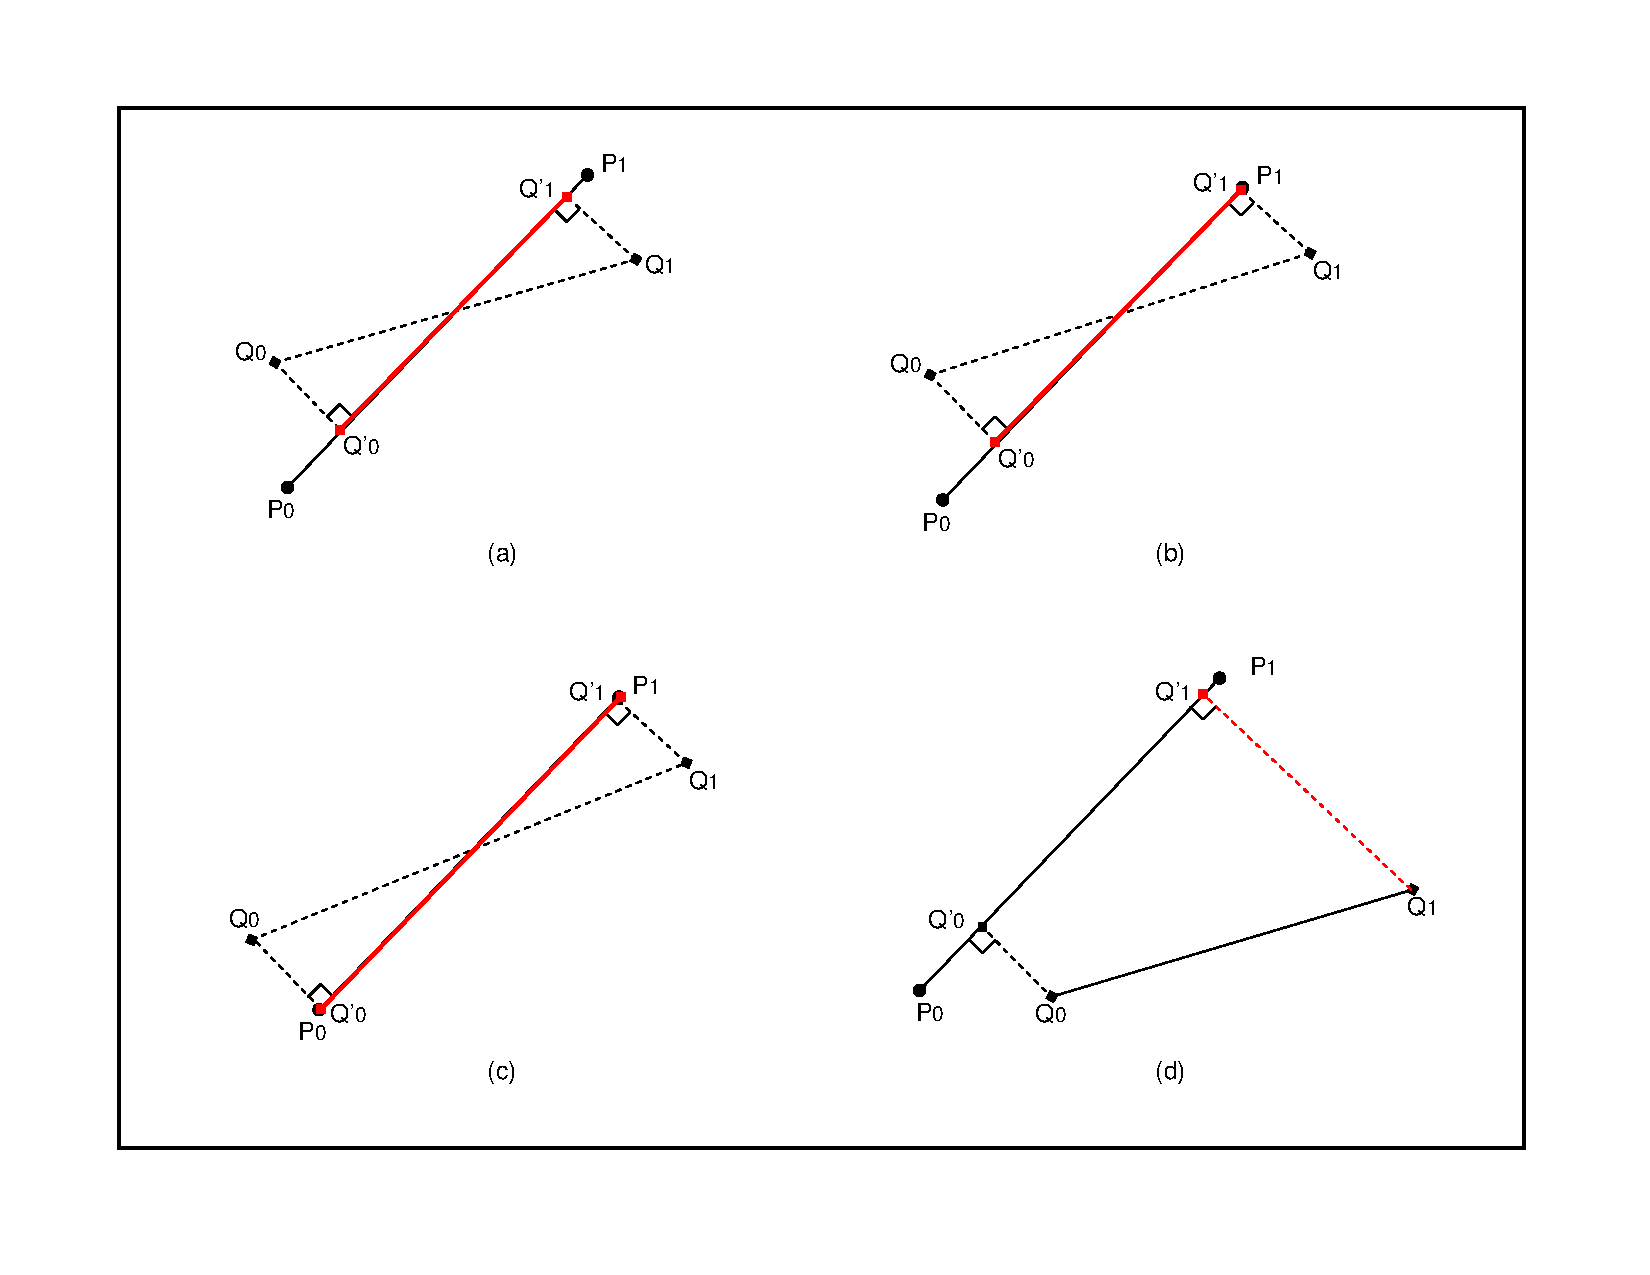
\includegraphics
      [width=\textwidth]
      {model_merge.pdf}
      \caption{Vertices adjustment for model merging
      (a) the two new points $Q_0$ and $Q_1$ are projected to an existed line as $Q'_0$ and $Q'_1$.
      (b) after (a), $Q'_1$ is merged with an existed point $P_1$.
      (c) after (a), both $Q'_0$ and $Q'_1$ are merged with existed point $P_0$ and $P_1$ respectively.
      (d) one of the point $Q_1$ is too far away for adjustment. }
      \label{fig:MR_Fig1}
\end{figure}

The first segmented part can be easily reconstructed without merging. 
Let ${\bf M}$ represent all lines or planes added into the final model so far. 
When adding a new line segment $Q_0Q_1$ to the model, 
we need to compute the closest line ${\bf L} = P_0P_1$ in ${\bf M}$ to $Q_0Q_1$.
Let $d = max(dist(Q_0, {\bf L}), dist(Q_1, {\bf L}))$, i.e., the larger distance 
between $Q_0$ to ${\bf L}$ and $Q_1$ to ${\bf L}$.
The distance from a point $Q$ to a line ${\bf L}$ can be computed using the equation:
\begin{equation*} % point to line equation
d(Q, { \bf L}) = | {\bf w - (w \cdot u) \, u} |
\end{equation*}
where ${\bf w} = (Q - P_0) $ and {\bf u} is the unit direction vector of {\bf L}.

There are several cases to be considered.
If $d <= \delta$, that is, both $Q_0$ and $Q_1$ are close enough to $L$, the projected point $Q'_0$ and $Q'_1$
are used to replace $Q_0$ and $Q_1$ respectively as shown in \Figa{MR_Fig1}. 
Furthermore, if one of the projected point, say $Q'_1$ is close to an end point of $L$, say $P_1$, 
$Q'_1$ would be merged with $P_1$ as shown in \Figb{MR_Fig1}. 
If both $Q'_0$ and $Q'_1$ are matched with $P_0$ and $P_1$, 
the line $Q_0Q_1$ would be merged totally with the line $L$, which was shown in \Figc{MR_Fig1}.
However, if $d > \delta$, no merging should be conducted as shown in \Figd{MR_Fig1}. 
\Figa{MR_Fig2} and \Figb{MR_Fig2} show the structures before and after model merge.


\begin{figure} [htbp]
\begin{center}
\begin{tabular}{cc}
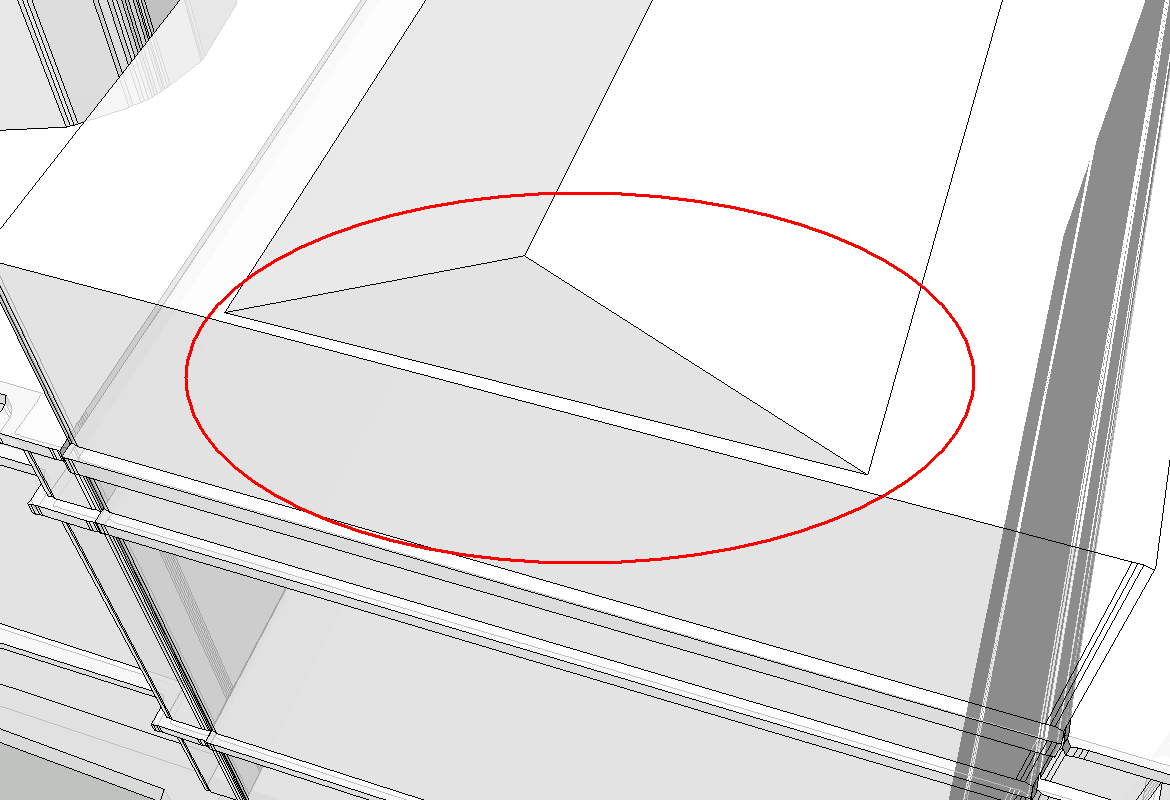
\includegraphics[width=0.45\textwidth]{model_before_merge.png} &
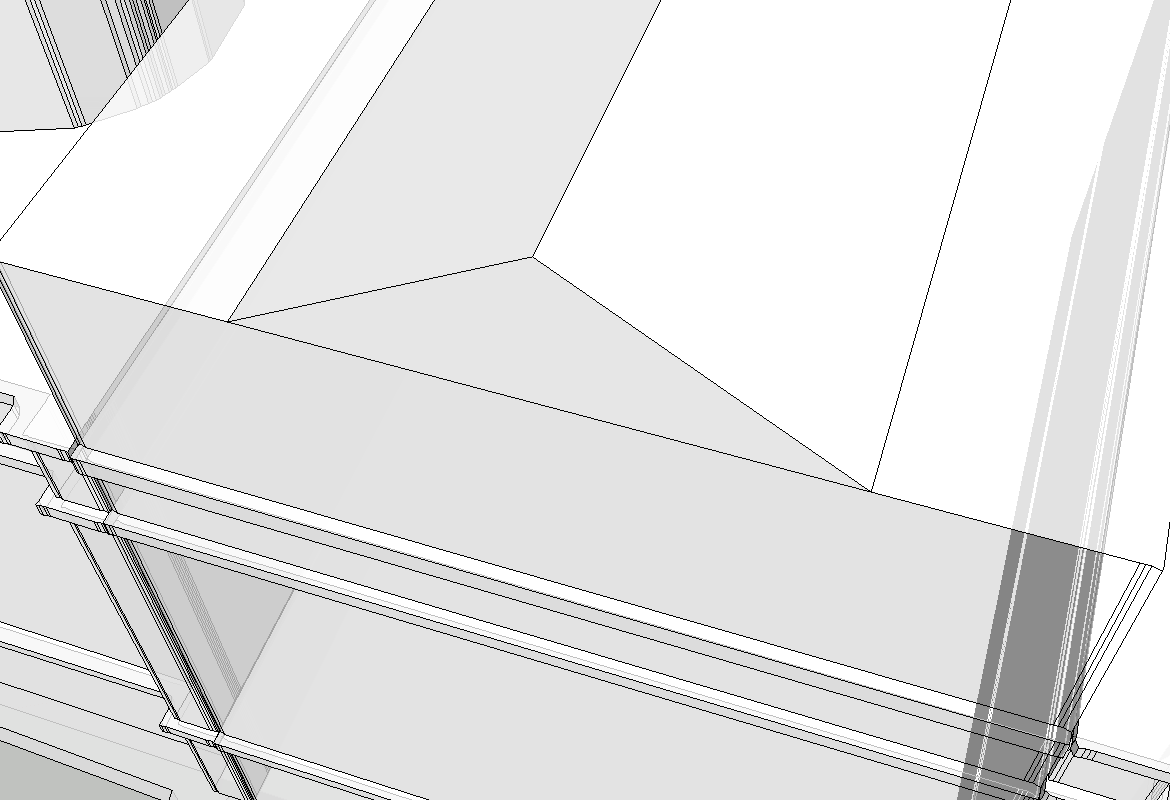
\includegraphics[width=0.45\textwidth]{model_after_merge.png} \\
(a) & (b) 
\end{tabular}
\end{center}
\caption{ 
      (a) two structures inside red ellipse are separated before merge
      (b) new structures after merge}
\label{fig:MR_Fig2}
\end{figure}

\section{Windows and Doors Installation}

After the model merging, the whole reconstructed model has been generated. 
We call this {\it naked} model in that there is no windows or doors yet as shown in \Figa{WDR_Fig1}.
If the point cloud contains windows or doors, we need to add them onto the naked model.
The window and door structures have been computed as described in Section \ref{sec:wdd},
now we need to know on which face or plane should they be added.

\begin{figure} [htbp]
\begin{center}
\begin{tabular}{cc}
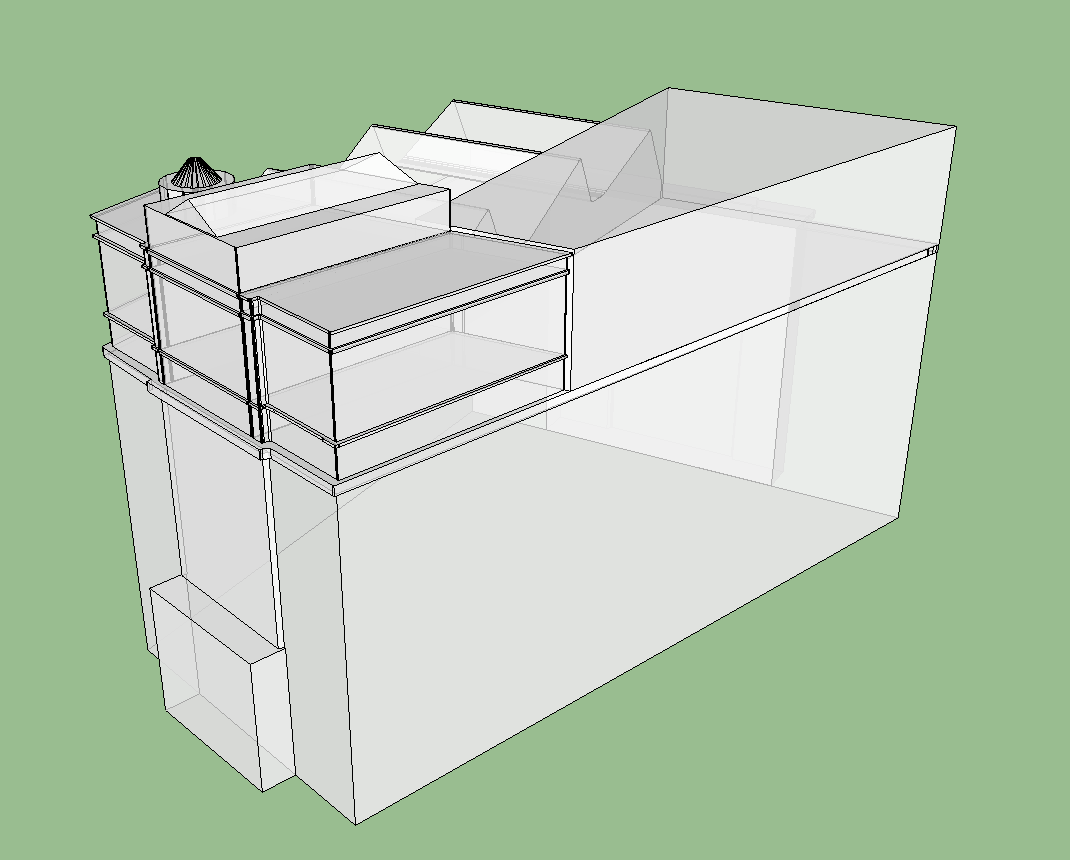
\includegraphics[width=0.45\textwidth]{model_naked.png} &
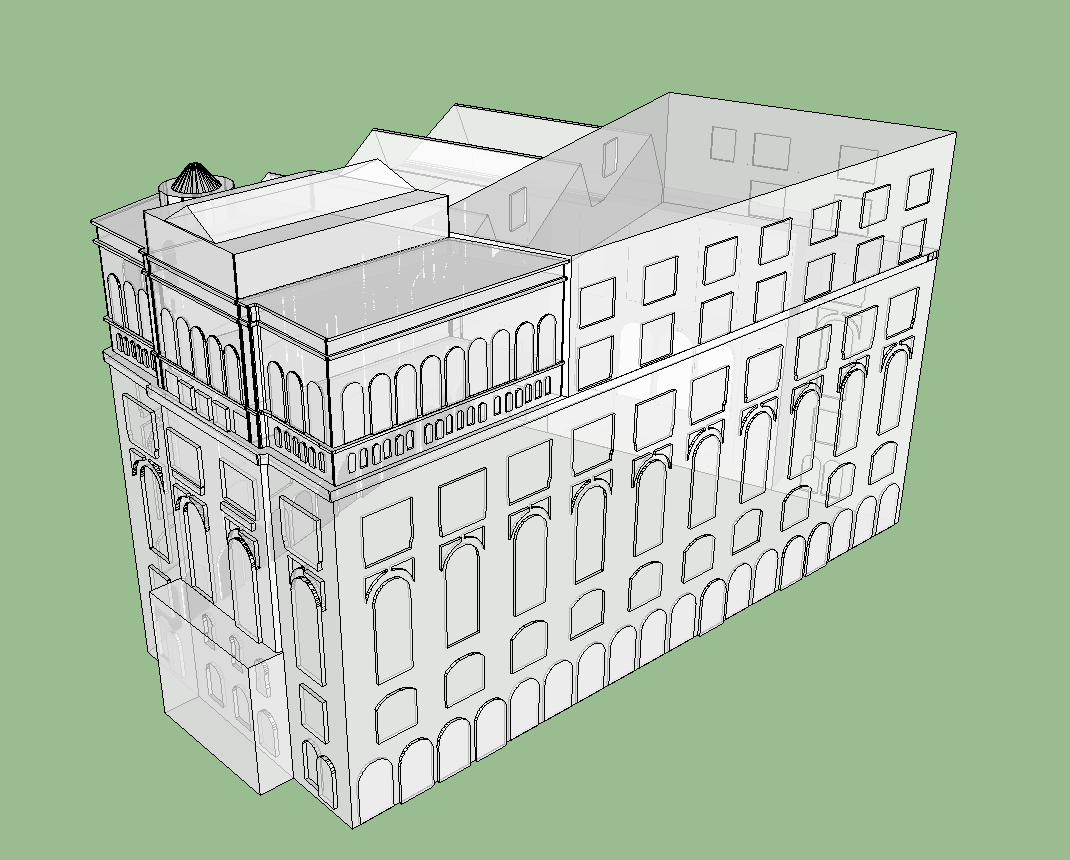
\includegraphics[width=0.45\textwidth]{model_windows.png} \\
(a) & (b) 
\end{tabular}
\end{center}
\caption{ Windows and doors reconstruction:
      (a) the reconstructed naked model.
      (b) the whole model with windows and doors added.}
\label{fig:WDR_Fig1}
\end{figure}

Let {\bf M} be the set of lines from a naked model.
Let $Q_0 = [X_{min}, Y_{min}], Q_1 = [X_{max}, Y_{max}]$ define the bounding box of a window $w$,
i.e., $[Q_0, Q_1]$ is the diagonal points for $w$.
Let $[Z_{min}, Z_{max}]$ be the height range of $w$.
The goal is to find the right face (closest line segment) for $w$ to be added.
For each line segment $L = P_0P_1 $ in ${\bf M}$, we first compute the projected points $Q'_0, Q'_1$
of $Q_0, Q_1$ on $L$ to check whether they are in between $[P_0, P_1]$. 
If not, $L$ is not eligible for adding $w$ since a window could not fall outside of a facade. 
Otherwise, the extruded range $L_{min}, L_{max}$ of $L$ is computed.
If $Z_{min} > L_{min}$ and $Z_{max} < L_{max}$, that is, the window $w$ is totally covered by the 
extruded face $F$ which is generated from $L$, $F$ is a potential face for adding $w$.
The distance $d_p = max(|Q_0Q'_0|, |Q_1Q'_1|)$ is used
to compare with global minimum distance $d_{p\_min}$ which was set to be a large value initially.
If $d_p < d_{p\_min}$, which means a closer face for $w$ is found, $d_{p\min}$ is updated to $d_p$ and
the corresponding line $L_{win}$ and its face $F_{win}$ are updated to $L$ and $F$ respectively. 

When all lines in ${\bf M}$ are checked, $F_{win}$ will give us the right face for adding $w$.
To add $w$ on $F_{win}$, we need to compute the projected point $P'$ for each vertex $P$ in $w$ on $F_{win}$.
Let $F_{win} = ax + by + cz + d$, the equation to compute $P(x_0, y_0, z_0)$ is
\begin{equation*} % projection point on a plane
P' = P - \frac{(ax_0+by_0+cz_0+d)}{a^2+b^2+c^2}\,{\bf n}
\end{equation*}
where {\bf n} is the normal of $F_{win}$.
This will generate a closed face $F_w$ on $F_{win}$. 
A simple push-pull operation on $F_w$ with the distance $d_w$ which was computed in the Section \ref{sec:wdd} 
will add the window $w$ onto $F_w$ of the naked model.
\Figb{WDR_Fig1} shows the entire model with windows and doors added for the model in \Figa{WDR_Fig1}.


\section{Experimental Results}

We have applied the proposed method on some synthetic datasets. The synthetic dataset were generated
from Sketchup models which were downloaded from Sketchup 3D warehouse. Essentially, the synthetic
dataset generator samples 3D point cloud data based on the face information extracted from the
Sketchup models. A parameter is used to control the sample rate of the face.

\Fig{ER_Fig1} through \Fig{ER_Fig10} shows the experimental results. For each set of the figures,
the original Sketchup model is shown in (a), the snapshot of the synthetic dataset sampled from (a)
is shown in (b). (c) and (d) shows the snapshots of the reconstructed model from different viewpoints.

However, there are some limitations on the proposed method. First of all, the error introduced in
early stages could be propagated to later stages, which could largely affect the final results.
For example, if the computation of the major faces introduces some errors and therefore the detected
the normals of the faces are not precise enough, the generation of the projected slices would be
problematic and the keyslices computation may be failed, which leads to the failure of the extrusion
structure detection.

Another limitation of the proposed method is that it could not handle the intersection of two
structures from different directions. For example, \Figa{ER_Lmt} shows a case where two extruded
structures intersect and \Figb{ER_Lmt} shows a case with intersection of a tapered structure and
an extruded structure. Both of them could not be handled by the proposed approach yet.

%% \begin{figure}[htbp]
%%   \centering
%%   \includegraphics
%%       [width=\textwidth]
%%       {expr_result1.pdf}
%%       \caption{Experimental Results of Cooper Union model:
%%       (a) original sketchup model.
%%       (b) synthetic point cloud data generated from (a).
%%       (c) reconstructed model (I) .
%%       (d) reconstructed model (II).}
%%       \label{fig:ER_Fig1}
%% \end{figure}
%%
%% \begin{figure}[htbp]
%%   \centering
%%   \includegraphics
%%       [width=\textwidth]
%%       {expr_result2.pdf}
%%       \caption{Experimental Results Spitak model:
%%       (a) original sketchup model.
%%       (b) synthetic point cloud data generated from (a).
%%       (c) reconstructed model (I) .
%%       (d) reconstructed model (II).}
%%       \label{fig:ER_Fig2}
%% \end{figure}
%%
%% \begin{figure}[htbp]
%%   \centering
%%   \includegraphics
%%       [width=\textwidth]
%%       {expr_result3.pdf}
%%       \caption{Experimental Results of house model:
%%       (a) original sketchup model.
%%       (b) synthetic point cloud data generated from (a).
%%       (c) reconstructed model (I) .
%%       (d) reconstructed model (II).}
%%       \label{fig:ER_Fig3}
%% \end{figure}
%%
%% \begin{figure}[htbp]
%%   \centering
%%   \includegraphics
%%       [width=\textwidth]
%%       {expr_result4.pdf}
%%       \caption{Experimental Results of Branch library model:
%%       (a) original sketchup model.
%%       (b) synthetic point cloud data generated from (a).
%%       (c) reconstructed model (I) .
%%       (d) reconstructed model (II).}
%%       \label{fig:ER_Fig4}
%% \end{figure}
%%
%% \begin{figure}[htbp]
%%   \centering
%%   \includegraphics
%%       [width=\textwidth]
%%       {expr_result5.pdf}
%%       \caption{Experimental Results of Clements library model:
%%       (a) original sketchup model.
%%       (b) synthetic point cloud data generated from (a).
%%       (c) reconstructed model (I) .
%%       (d) reconstructed model (II).}
%%       \label{fig:ER_Fig5}
%% \end{figure}
%%
%% \begin{figure}[htbp]
%%   \centering
%%   \includegraphics
%%       [width=\textwidth]
%%       {expr_result6.pdf}
%%       \caption{Experimental Results of Doe library model:
%%       (a) original sketchup model.
%%       (b) synthetic point cloud data generated from (a).
%%       (c) reconstructed model (I) .
%%       (d) reconstructed model (II).}
%%       \label{fig:ER_Fig6}
%% \end{figure}
%%
%% \begin{figure}[htbp]
%%   \centering
%%   \includegraphics
%%       [width=\textwidth]
%%       {expr_result7.pdf}
%%       \caption{Experimental Results of Health Town library model:
%%       (a) original sketchup model.
%%       (b) synthetic point cloud data generated from (a).
%%       (c) reconstructed model (I) .
%%       (d) reconstructed model (II).}
%%       \label{fig:ER_Fig7}
%% \end{figure}
%%
%% \begin{figure}[htbp]
%%   \centering
%%   \includegraphics
%%       [width=\textwidth]
%%       {expr_result8.pdf}
%%       \caption{Experimental Results of Miami Date Court model:
%%       (a) original sketchup model.
%%       (b) synthetic point cloud data generated from (a).
%%       (c) reconstructed model (I) .
%%       (d) reconstructed model (II).}
%%       \label{fig:ER_Fig8}
%% \end{figure}
%%
%% \begin{figure}[htbp]
%%   \centering
%%   \includegraphics
%%       [width=\textwidth]
%%       {expr_result9.pdf}
%%       \caption{Experimental Results of simple model:
%%       (a) original sketchup model.
%%       (b) synthetic point cloud data generated from (a).
%%       (c) reconstructed model (I) .
%%       (d) reconstructed model (II).}
%%       \label{fig:ER_Fig9}
%% \end{figure}
%%
%% \begin{figure}[htbp]
%%   \centering
%%   \includegraphics
%%       [width=\textwidth]
%%       {expr_result10.pdf}
%%       \caption{Experimental Results of St Michael church model:
%%       (a) original sketchup model.
%%       (b) synthetic point cloud data generated from (a).
%%       (c) reconstructed model (I) .
%%       (d) reconstructed model (II).}
%%       \label{fig:ER_Fig10}
%% \end{figure}

\begin{figure} [htbp]
\begin{center}
\begin{tabular}{cc}
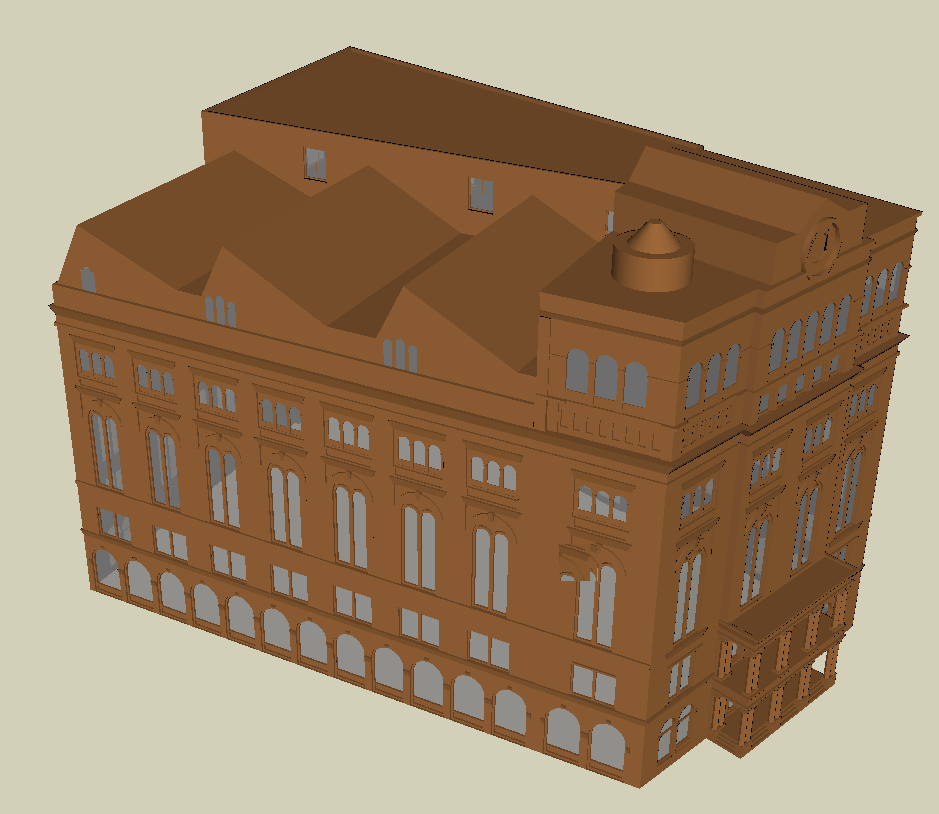
\includegraphics[width=0.5\textwidth]{cu_1.png} &
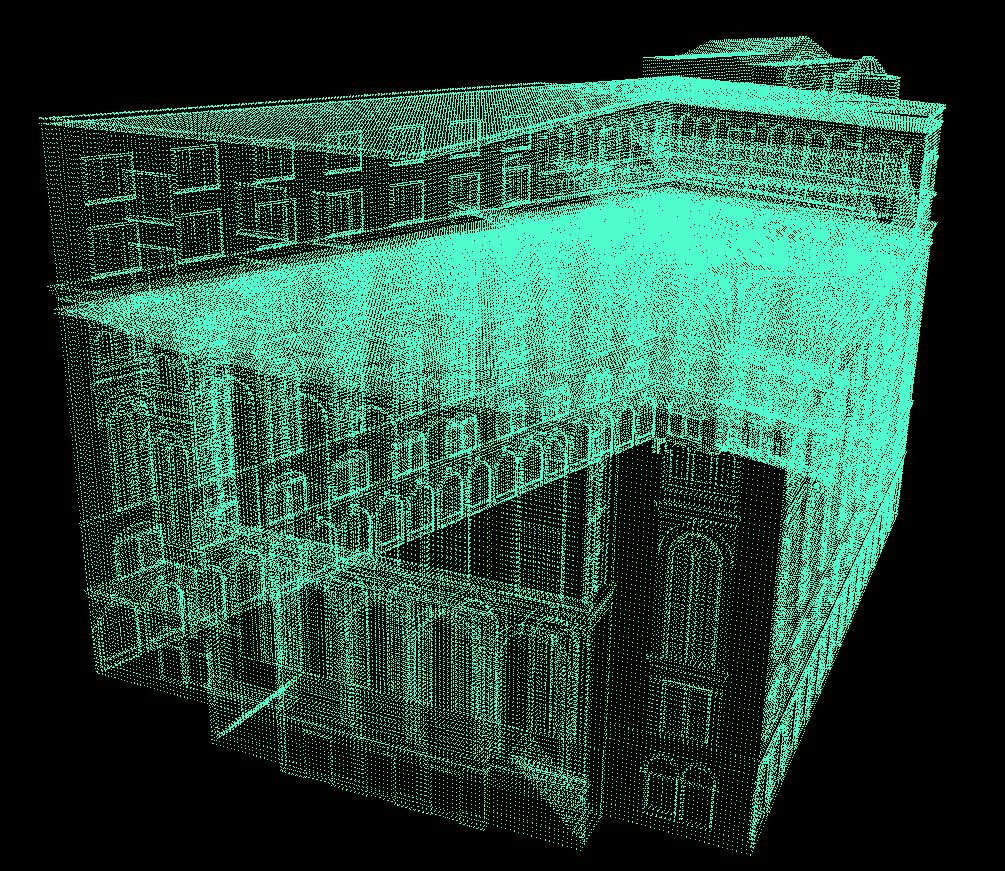
\includegraphics[width=0.5\textwidth]{cu_2.png} \\
(a) & (b) \\
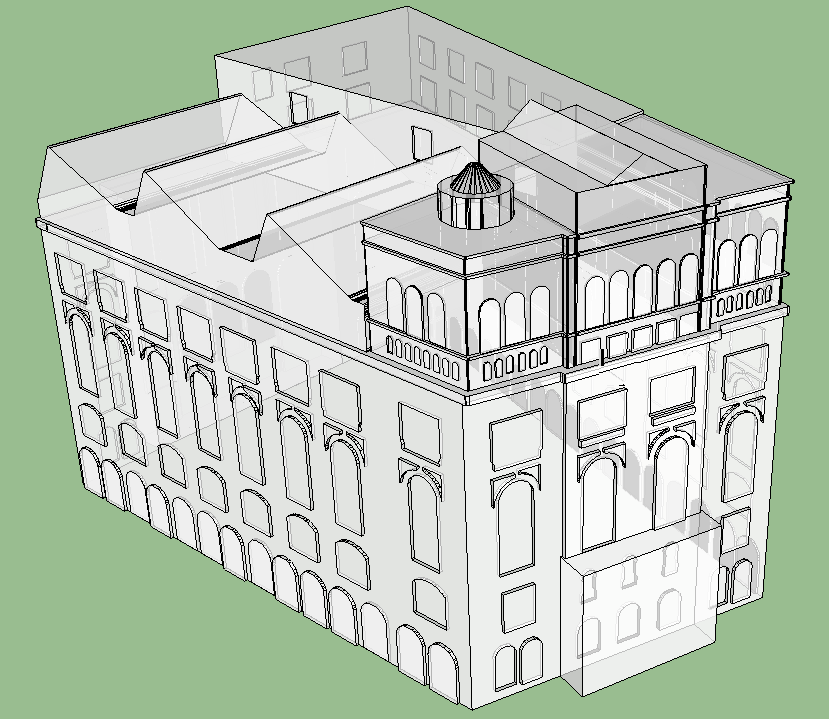
\includegraphics[width=0.5\textwidth]{cu_3.png} &
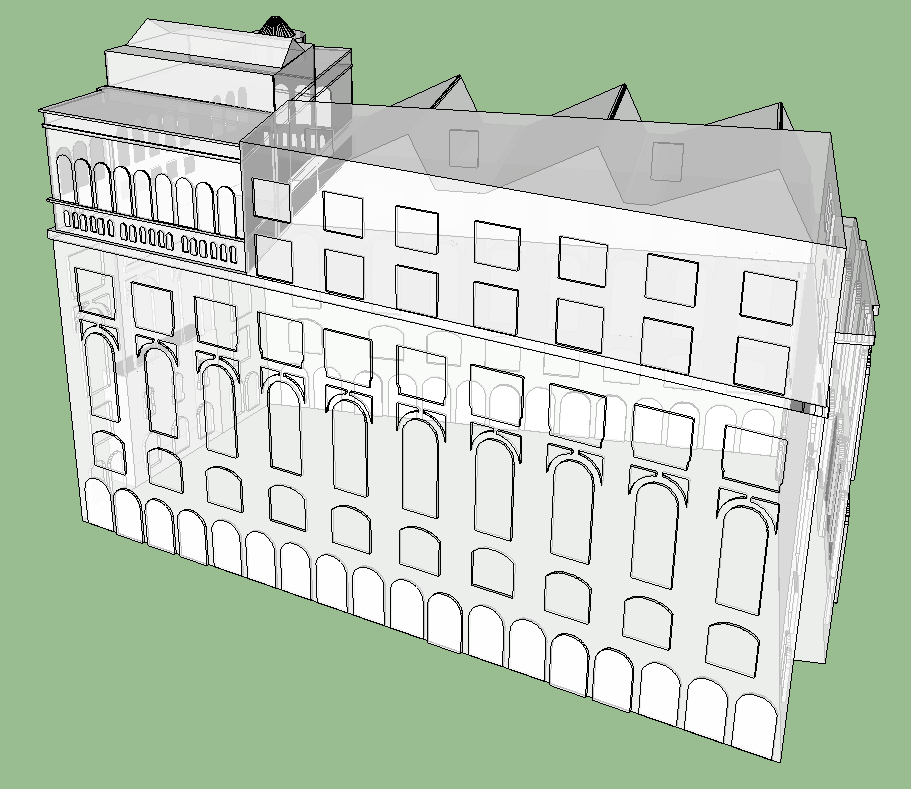
\includegraphics[width=0.5\textwidth]{cu_4.png} \\
(c) & (d)
\end{tabular}
\end{center}
\caption{Experimental Results of Cooper Union model:
      (a) original Sketchup model.
      (b) synthetic point cloud data generated from (a).
      (c) reconstructed model (I) .
      (d) reconstructed model (II).}
\label{fig:ER_Fig1}
\end{figure}

\begin{figure} [htbp]
\begin{center}
\begin{tabular}{cc}
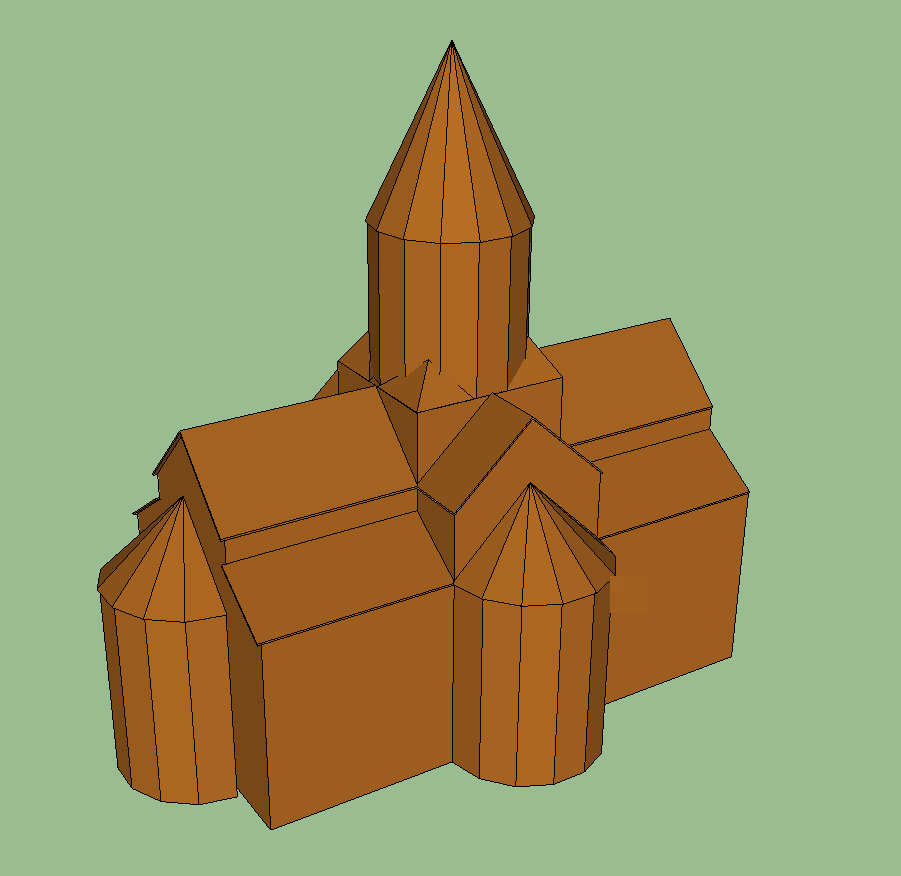
\includegraphics[width=0.5\textwidth]{spitak_1.png} &
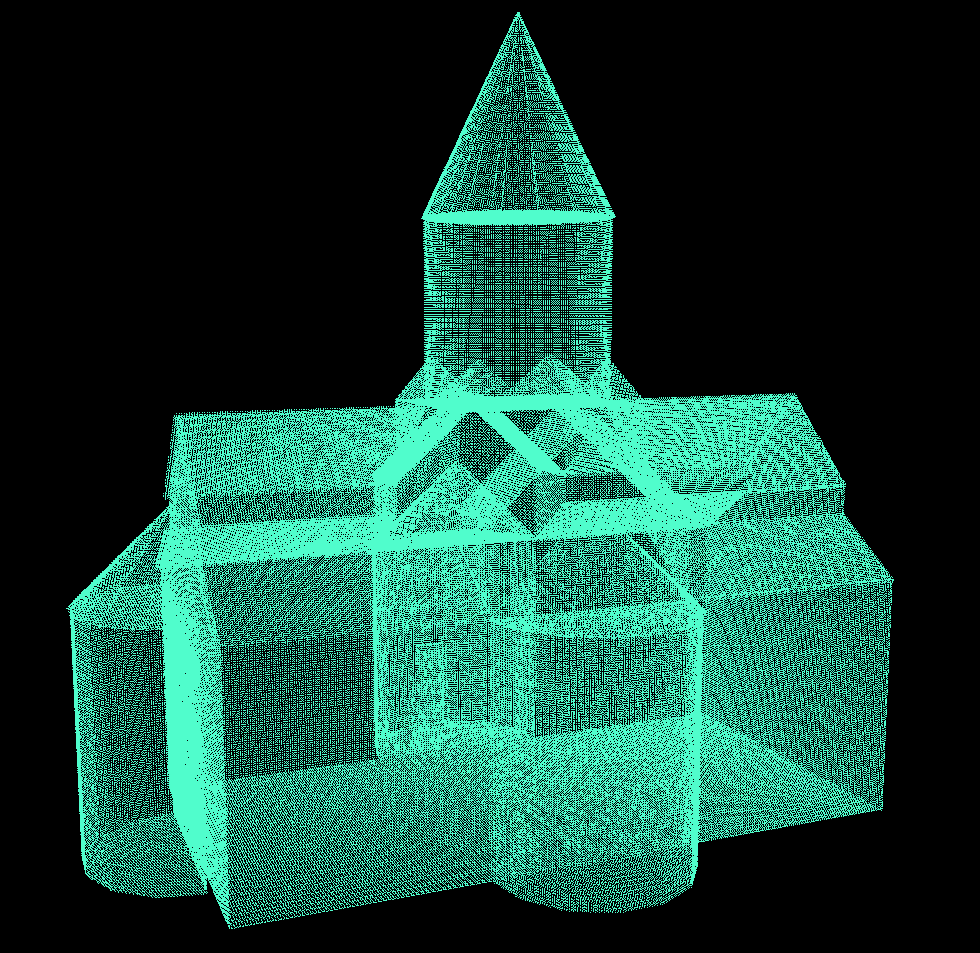
\includegraphics[width=0.5\textwidth]{spitak_2.png} \\
(a) & (b) \\
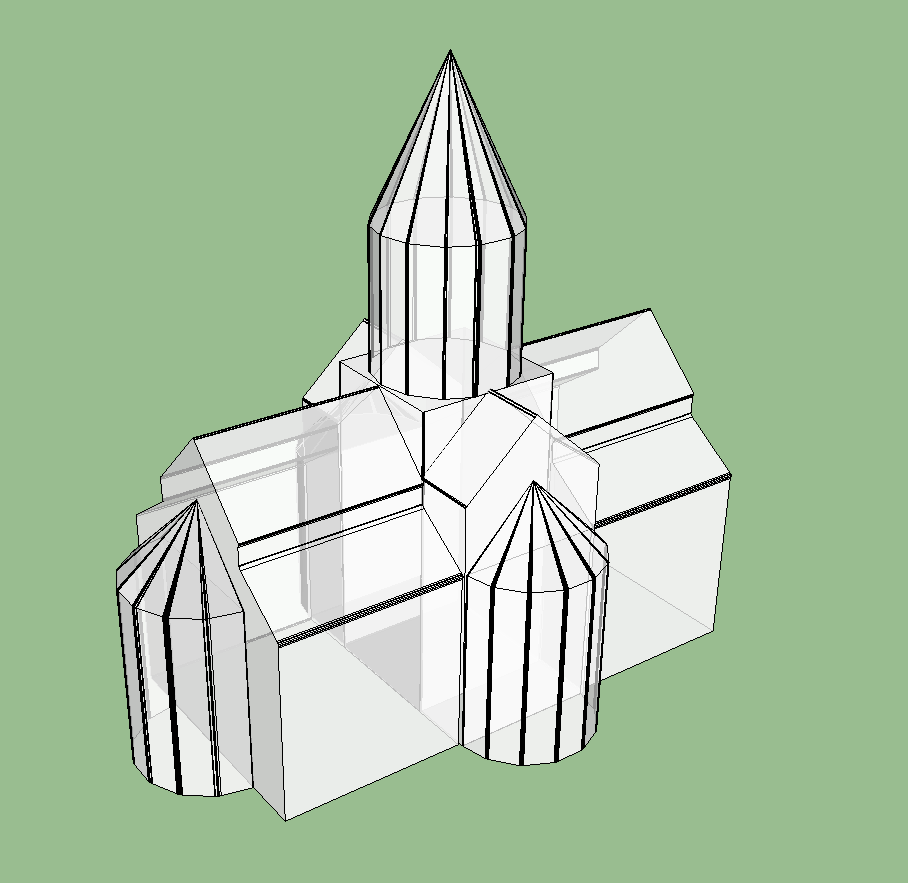
\includegraphics[width=0.5\textwidth]{spitak_3.png} &
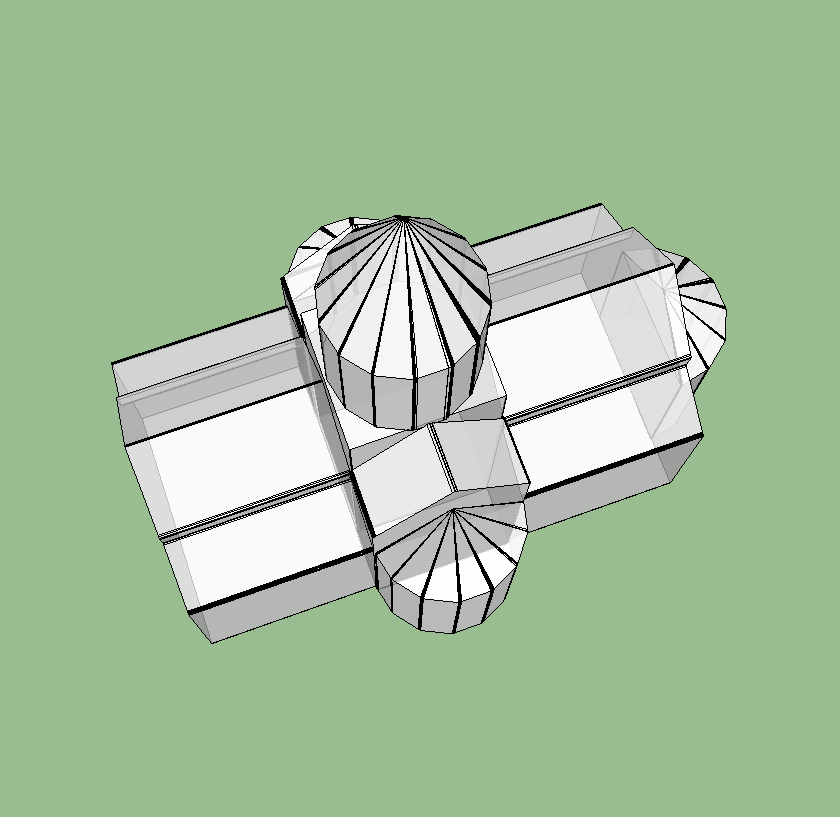
\includegraphics[width=0.5\textwidth]{spitak_4.png} \\
(c) & (d)
\end{tabular}
\end{center}
\caption{Experimental Results of Spitak model:
      (a) original Sketchup model.
      (b) synthetic point cloud data generated from (a).
      (c) reconstructed model (I) .
      (d) reconstructed model (II).}
\label{fig:ER_Fig2}
\end{figure}

\begin{figure} [htbp]
\begin{center}
\begin{tabular}{cc}
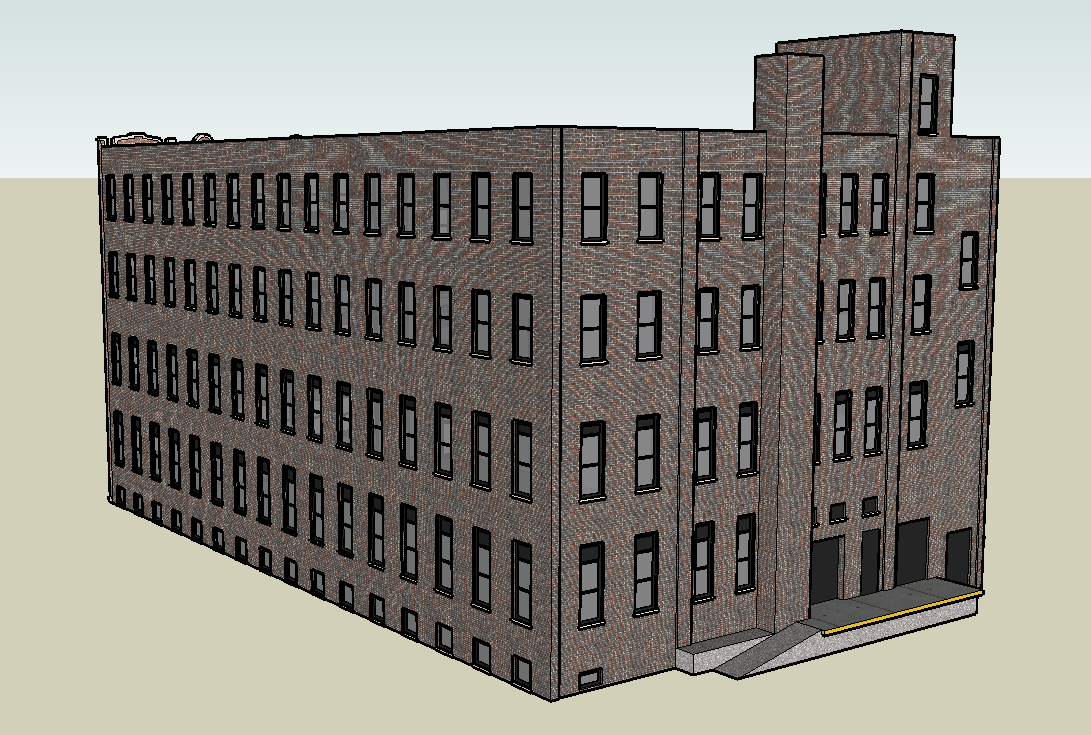
\includegraphics[width=0.5\textwidth]{house_1.png} &
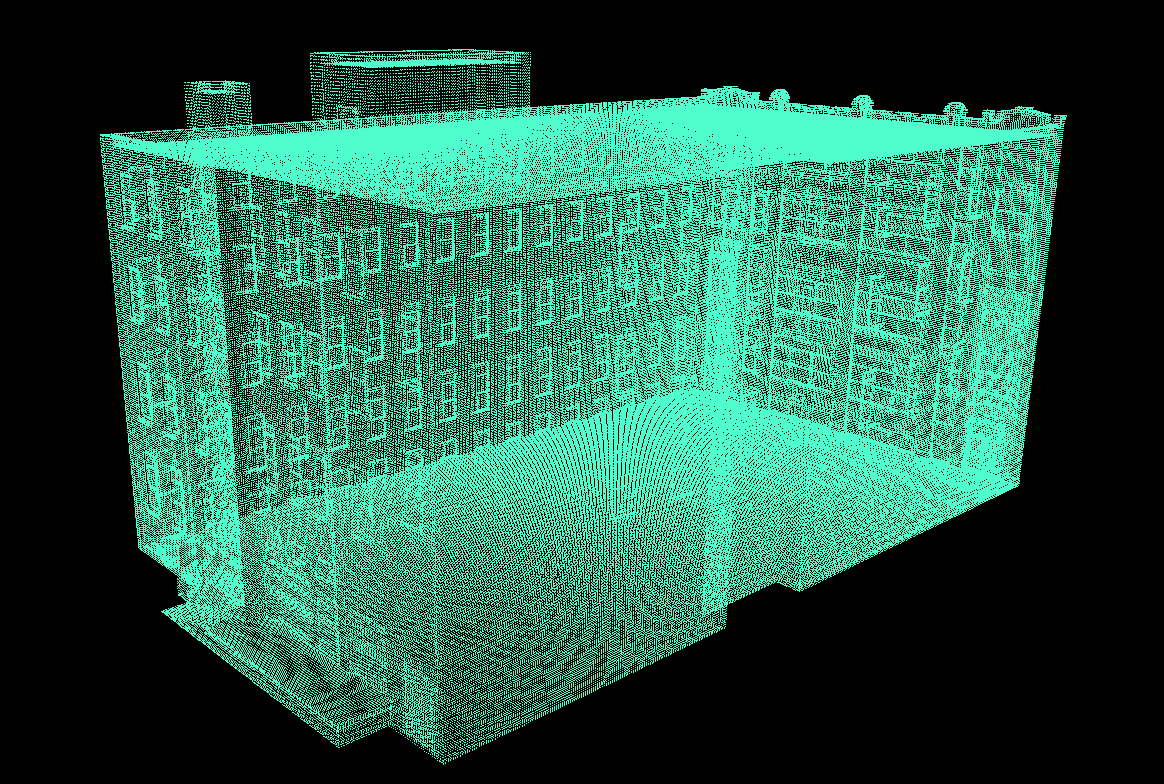
\includegraphics[width=0.5\textwidth]{house_2.png} \\
(a) & (b) \\
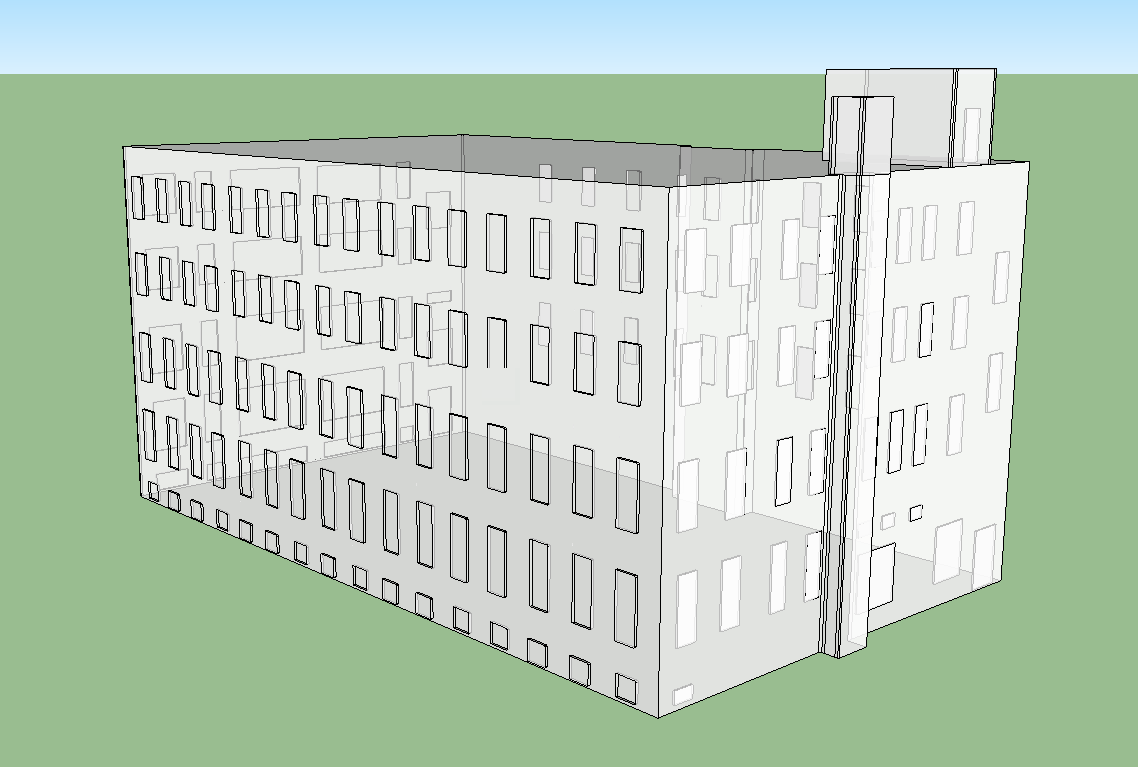
\includegraphics[width=0.5\textwidth]{house_3.png} &
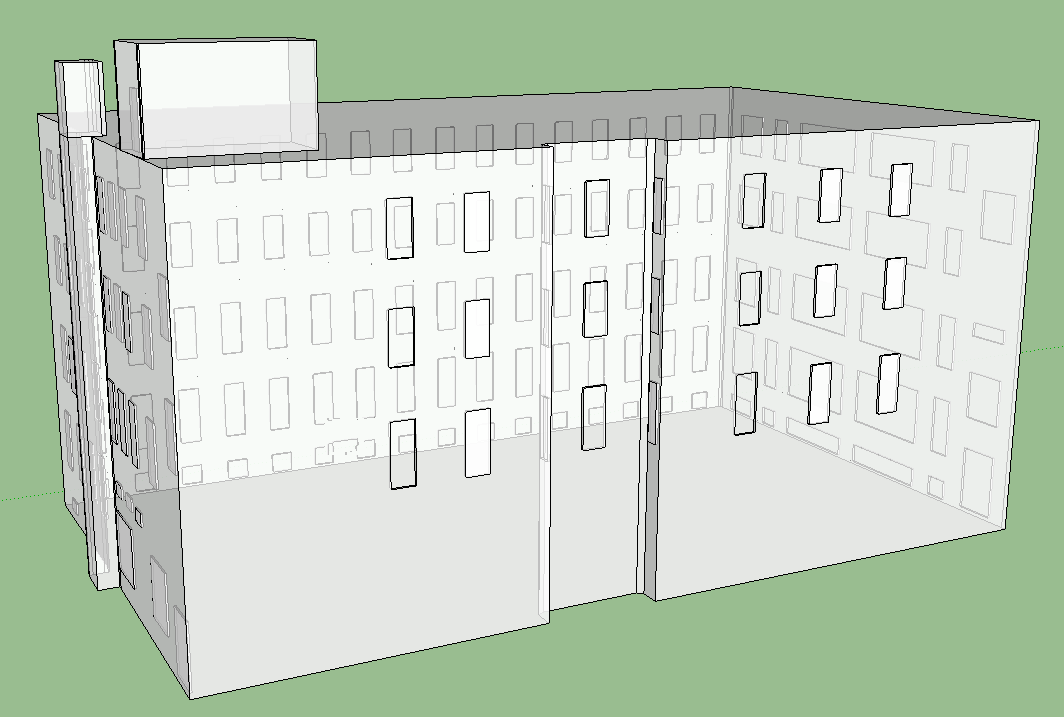
\includegraphics[width=0.5\textwidth]{house_4.png} \\
(c) & (d)
\end{tabular}
\end{center}
\caption{Experimental Results of house model:
      (a) original Sketchup model.
      (b) synthetic point cloud data generated from (a).
      (c) reconstructed model (I) .
      (d) reconstructed model (II).}
\label{fig:ER_Fig3}
\end{figure}

\begin{figure} [htbp]
\begin{center}
\begin{tabular}{cc}
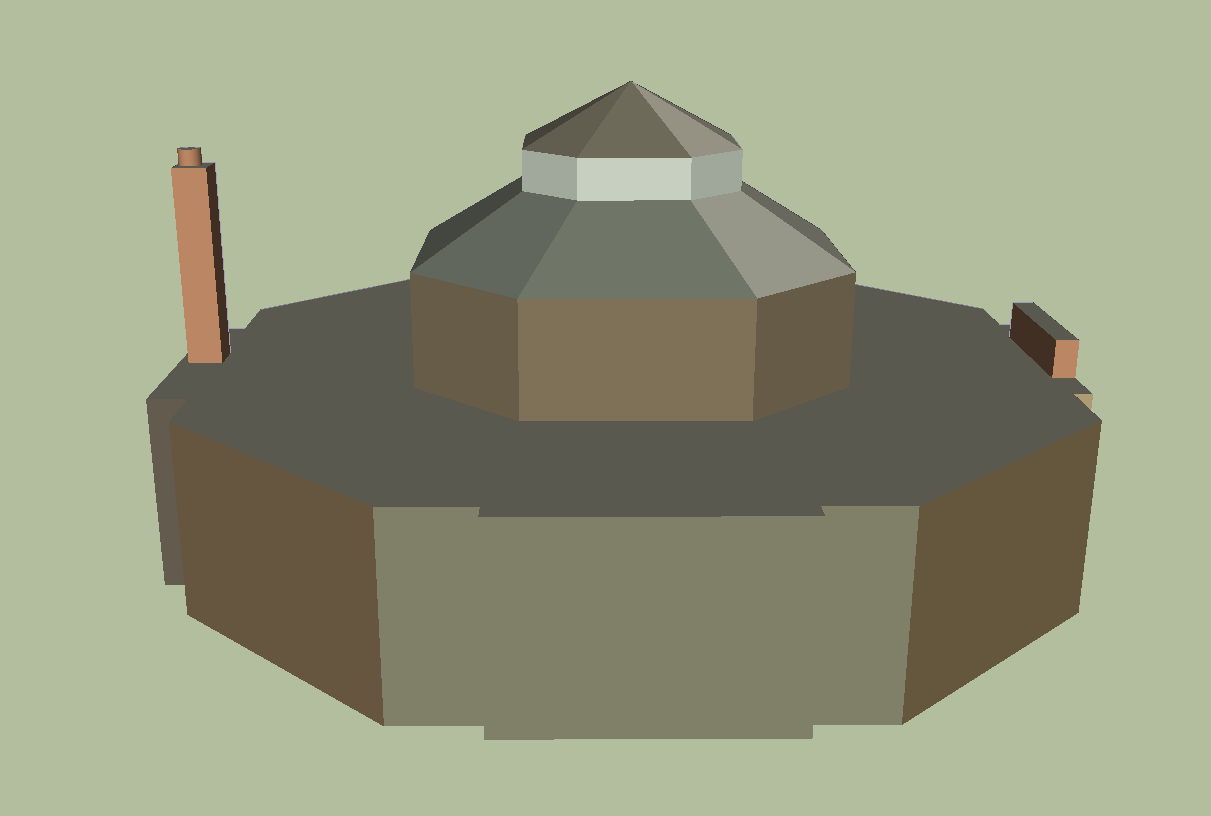
\includegraphics[width=0.5\textwidth]{branch_lib_1.png} &
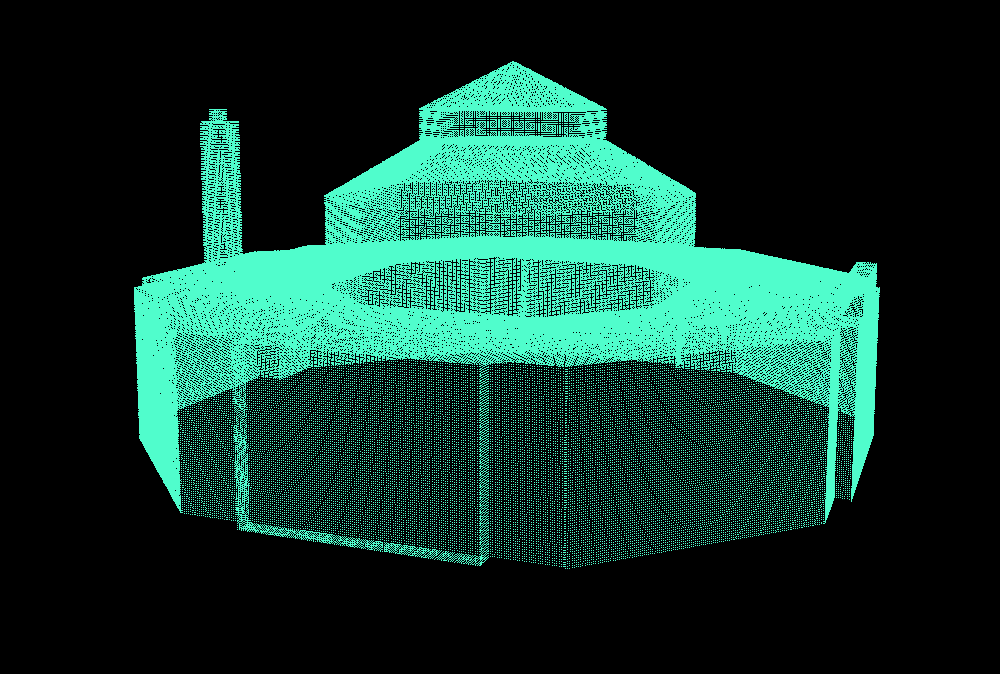
\includegraphics[width=0.5\textwidth]{branch_lib_2.png} \\
(a) & (b) \\
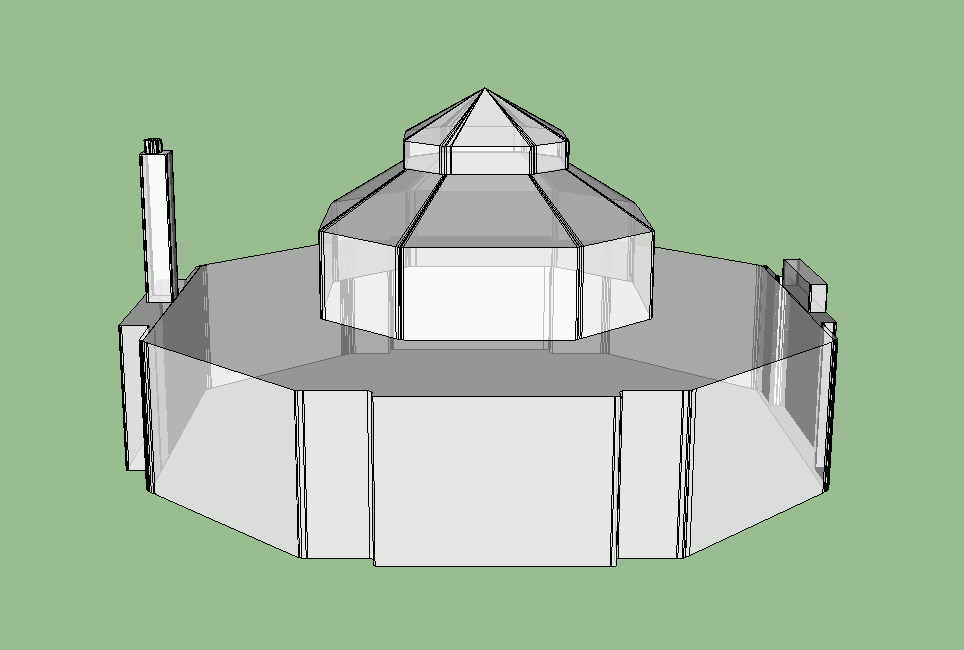
\includegraphics[width=0.5\textwidth]{branch_lib_3.png} &
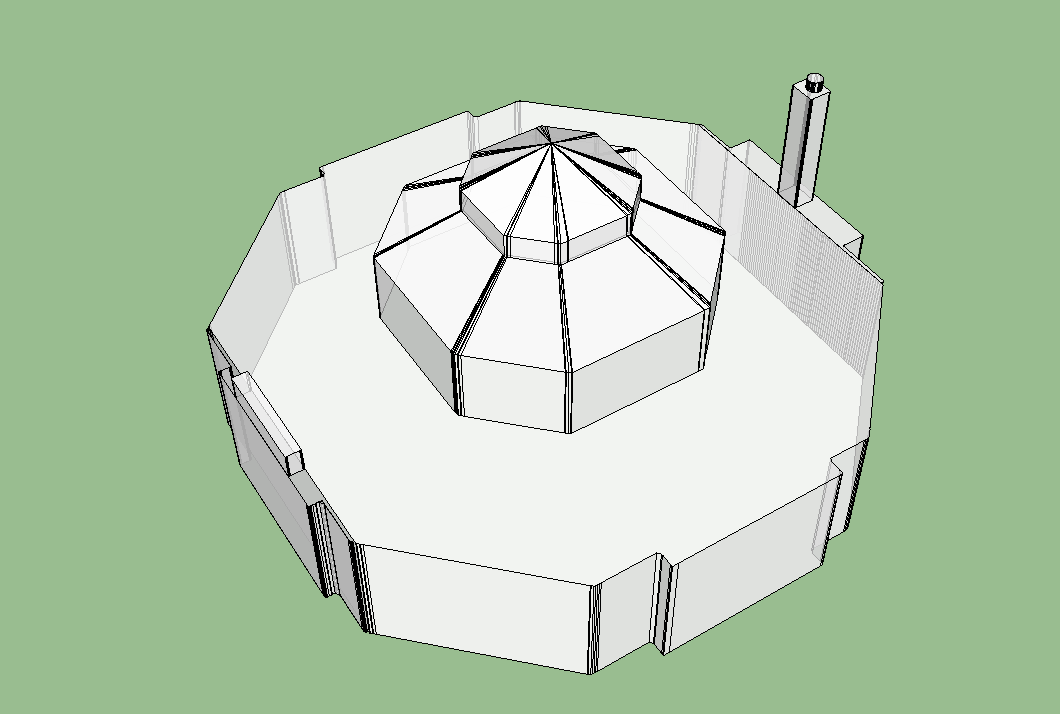
\includegraphics[width=0.5\textwidth]{branch_lib_4.png} \\
(c) & (d)
\end{tabular}
\end{center}
\caption{Experimental Results of Branch library model:
      (a) original Sketchup model.
      (b) synthetic point cloud data generated from (a).
      (c) reconstructed model (I) .
      (d) reconstructed model (II).}
\label{fig:ER_Fig4}
\end{figure}

\begin{figure} [htbp]
\begin{center}
\begin{tabular}{cc}
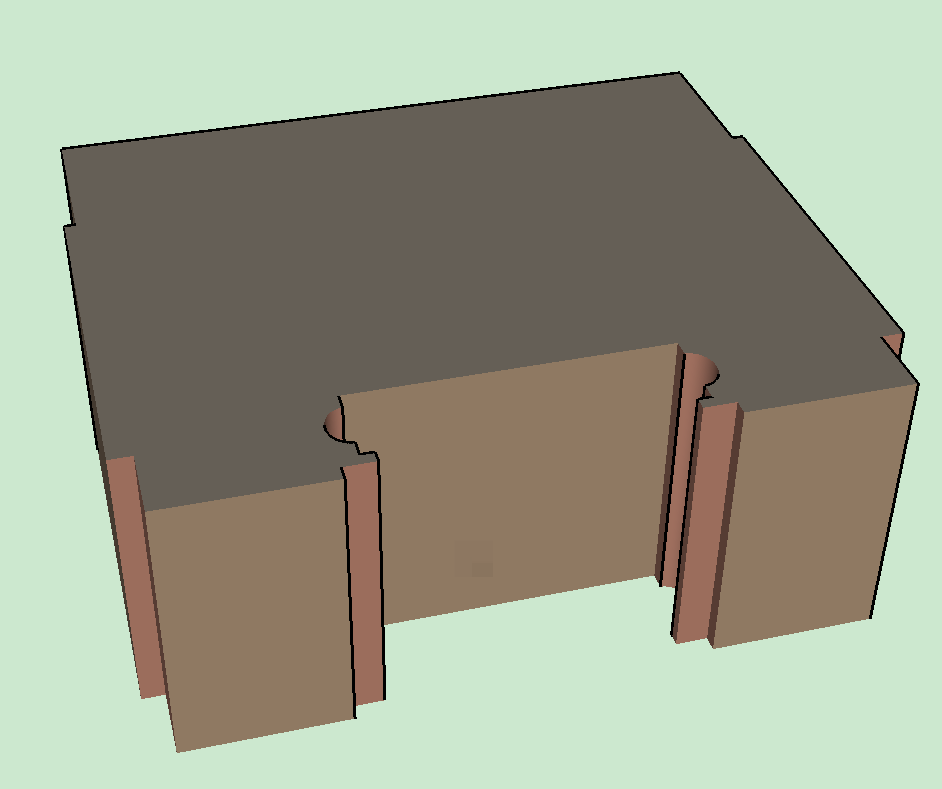
\includegraphics[width=0.5\textwidth]{clements_lib_1.png} &
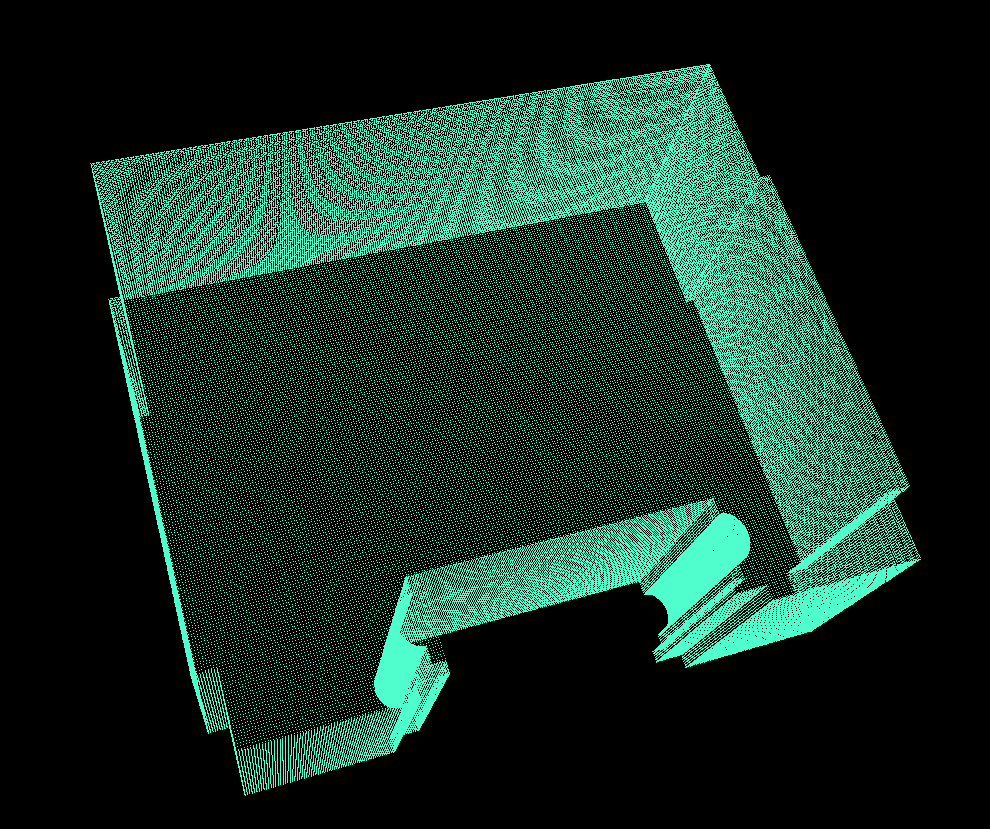
\includegraphics[width=0.5\textwidth]{clements_lib_2.png} \\
(a) & (b) \\
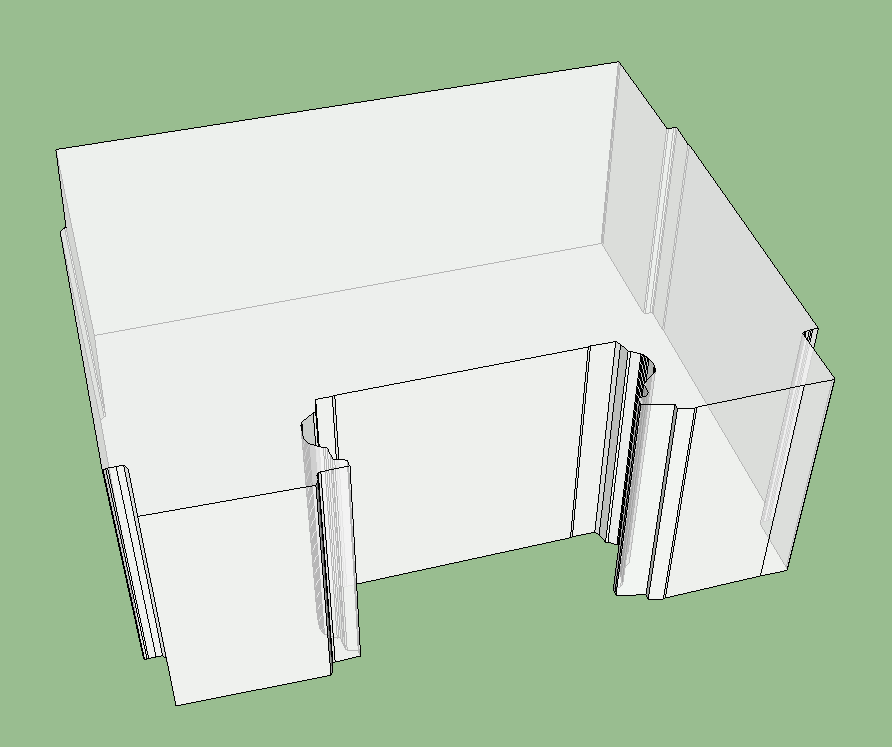
\includegraphics[width=0.5\textwidth]{clements_lib_3.png} &
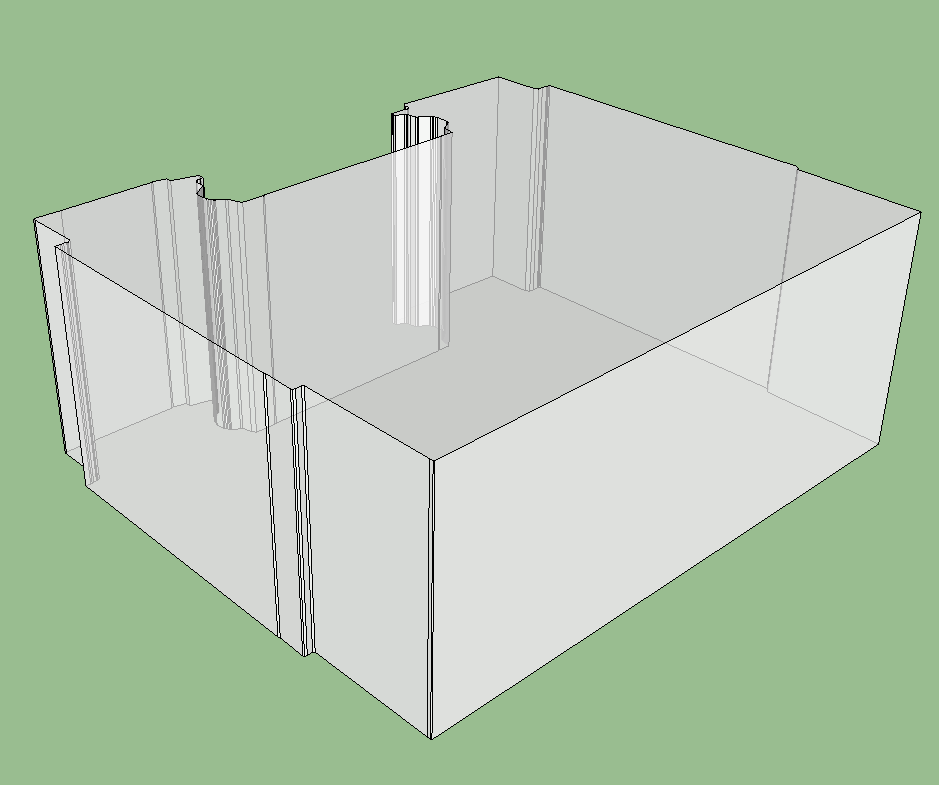
\includegraphics[width=0.5\textwidth]{clements_lib_4.png} \\
(c) & (d)
\end{tabular}
\end{center}
\caption{Experimental Results of Clements library model:
      (a) original Sketchup model.
      (b) synthetic point cloud data generated from (a).
      (c) reconstructed model (I) .
      (d) reconstructed model (II).}
\label{fig:ER_Fig5}
\end{figure}

\begin{figure} [htbp]
\begin{center}
\begin{tabular}{cc}
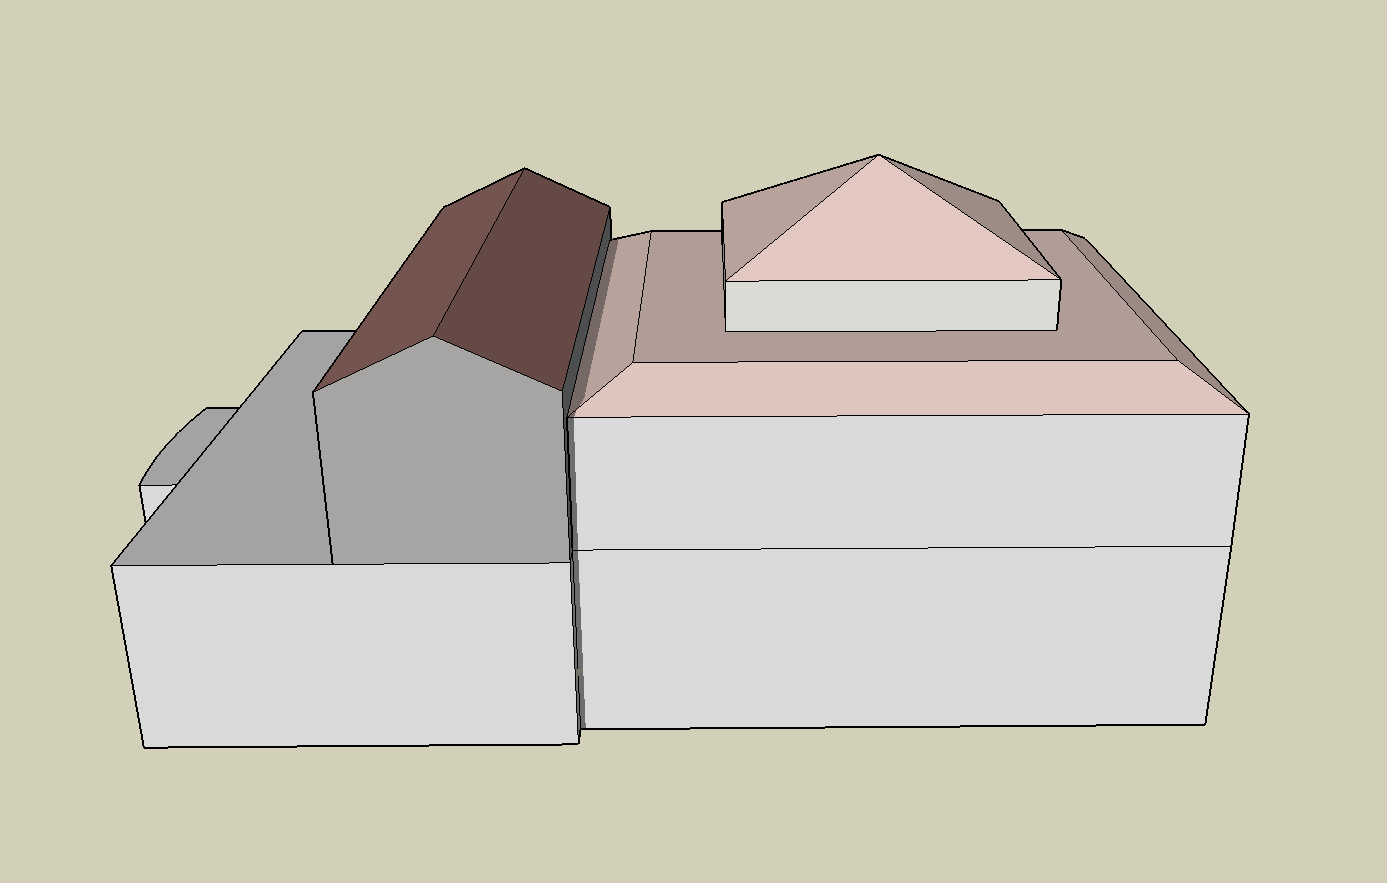
\includegraphics[width=0.5\textwidth]{doe_1.png} &
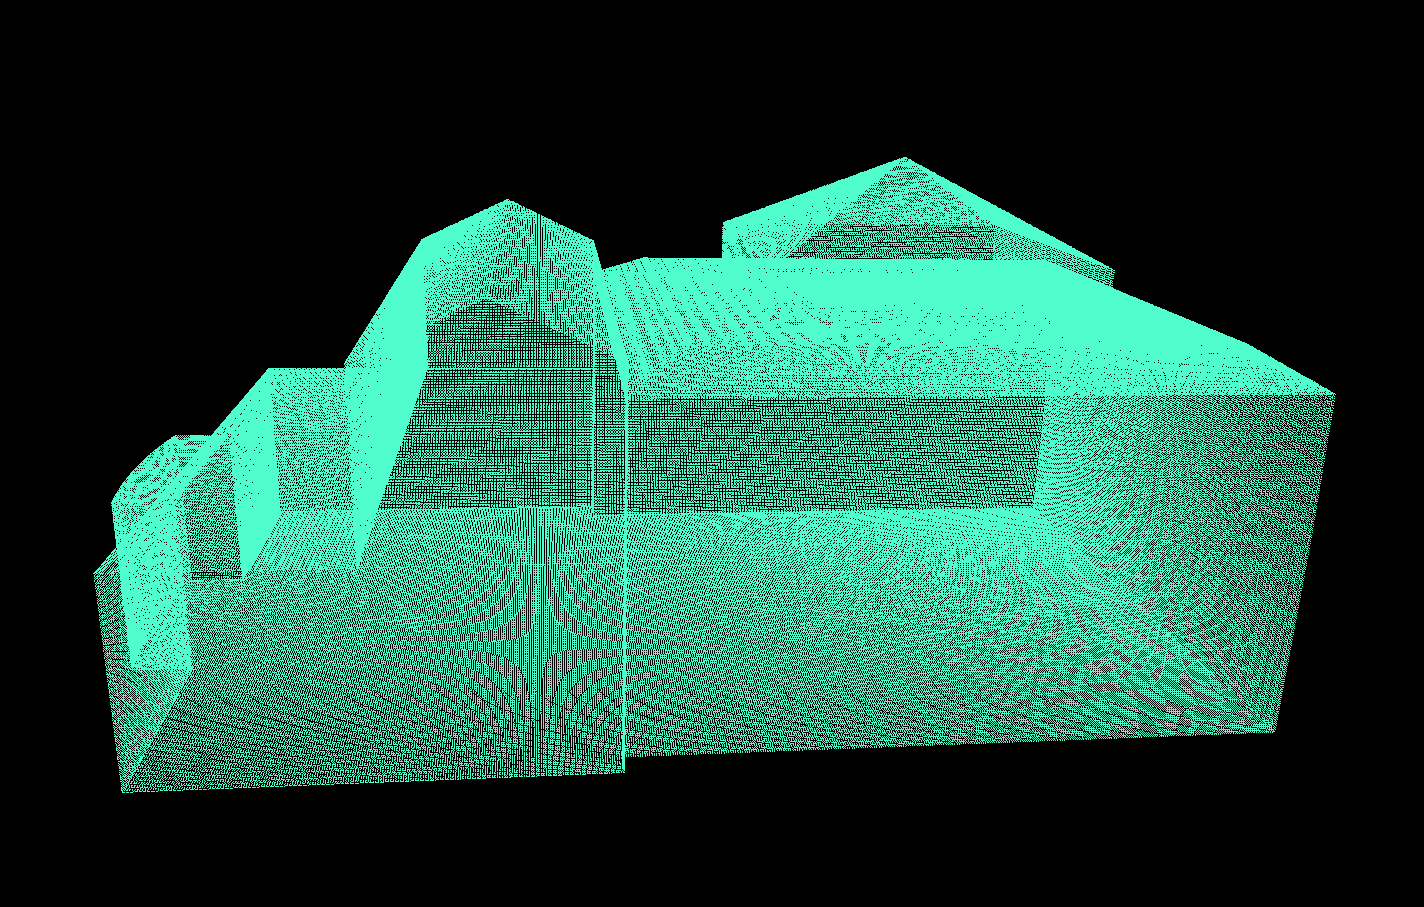
\includegraphics[width=0.5\textwidth]{doe_2.png} \\
(a) & (b) \\
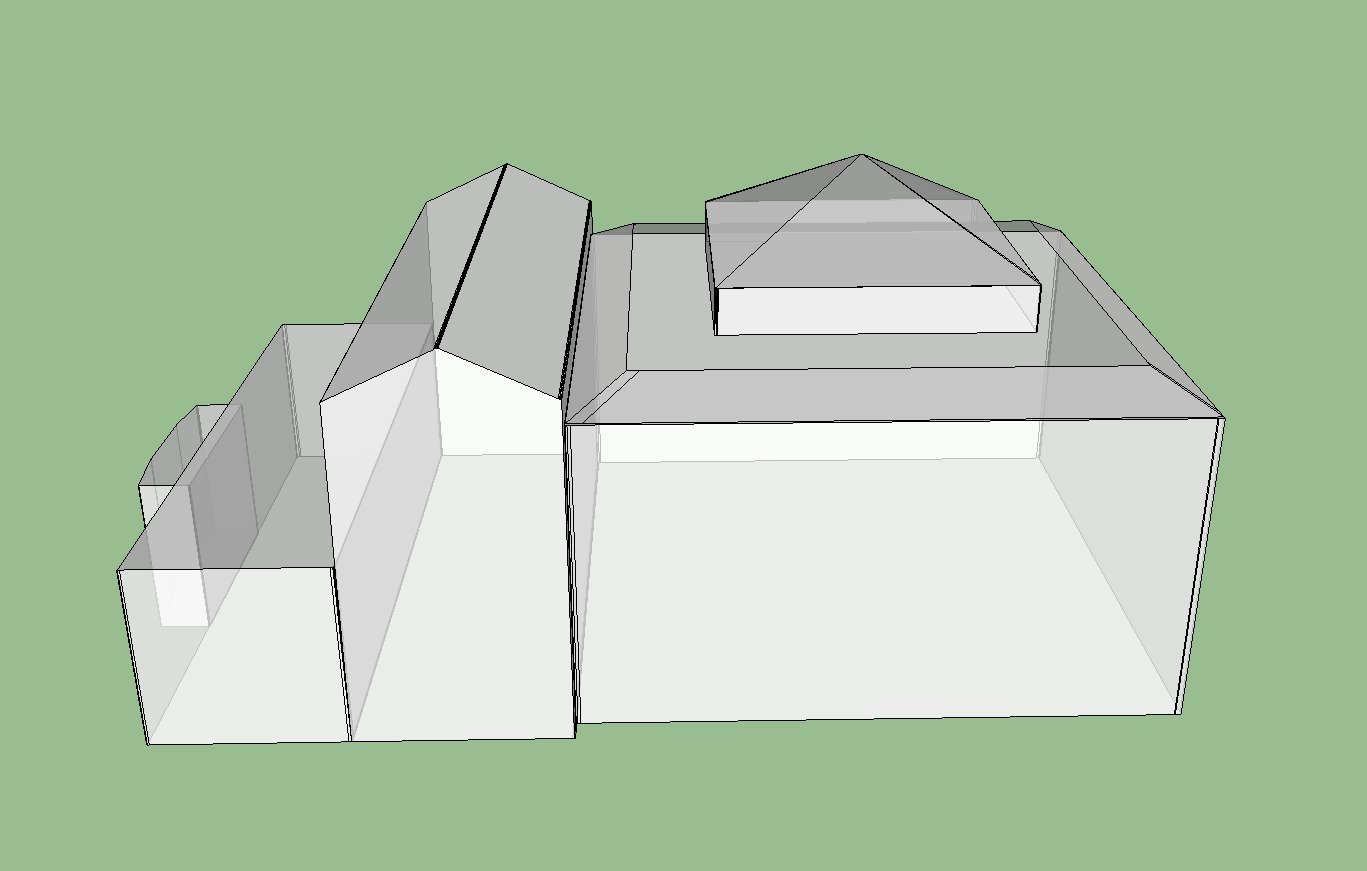
\includegraphics[width=0.5\textwidth]{doe_3.png} &
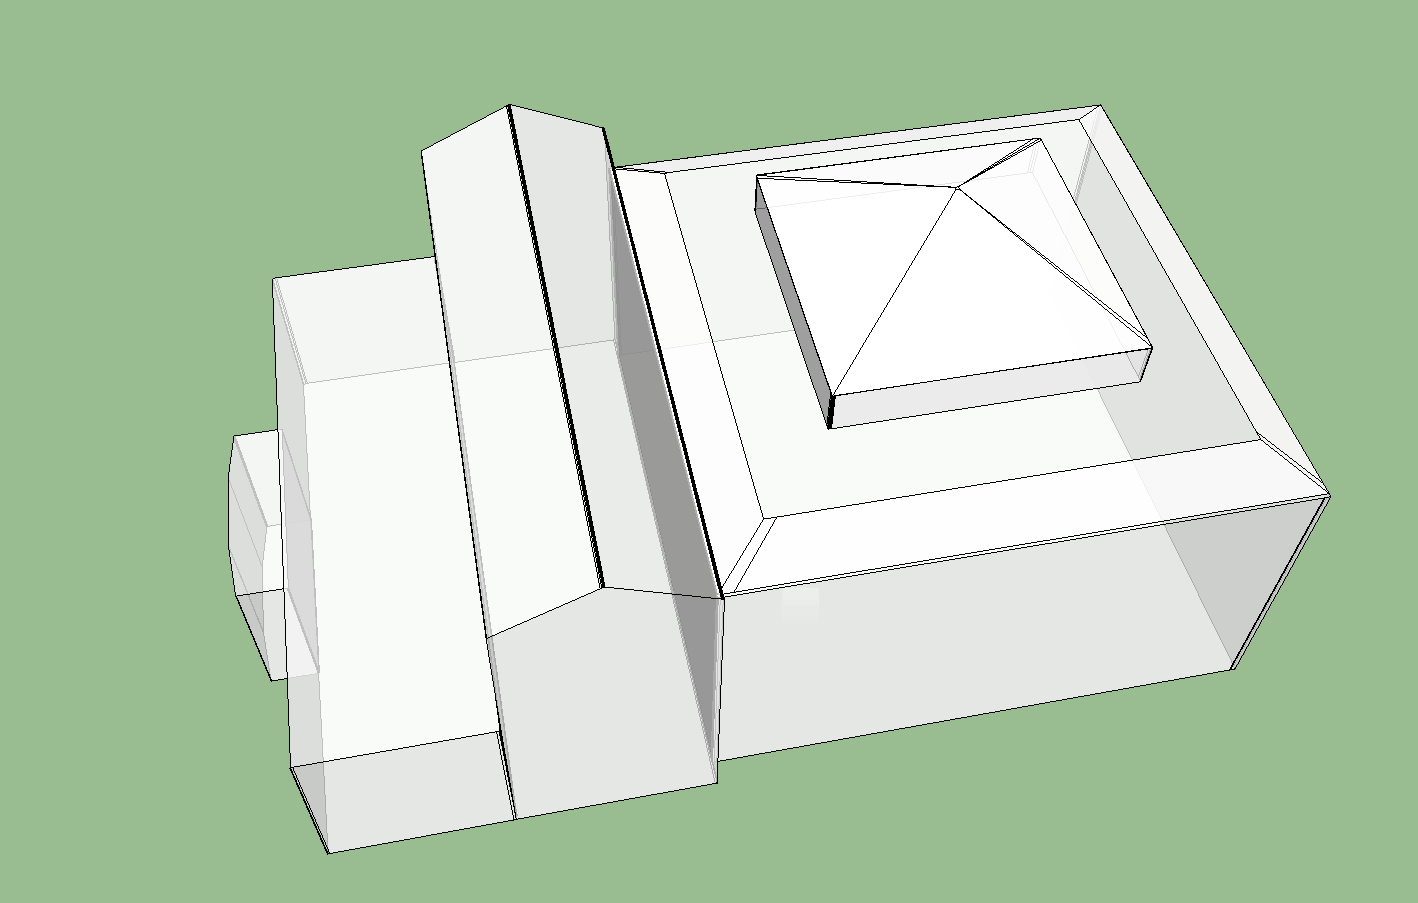
\includegraphics[width=0.5\textwidth]{doe_4.png} \\
(c) & (d)
\end{tabular}
\end{center}
\caption{Experimental Results of Doe library model:
      (a) original Sketchup model.
      (b) synthetic point cloud data generated from (a).
      (c) reconstructed model (I) .
      (d) reconstructed model (II).}
\label{fig:ER_Fig6}
\end{figure}

\begin{figure} [htbp]
\begin{center}
\begin{tabular}{cc}
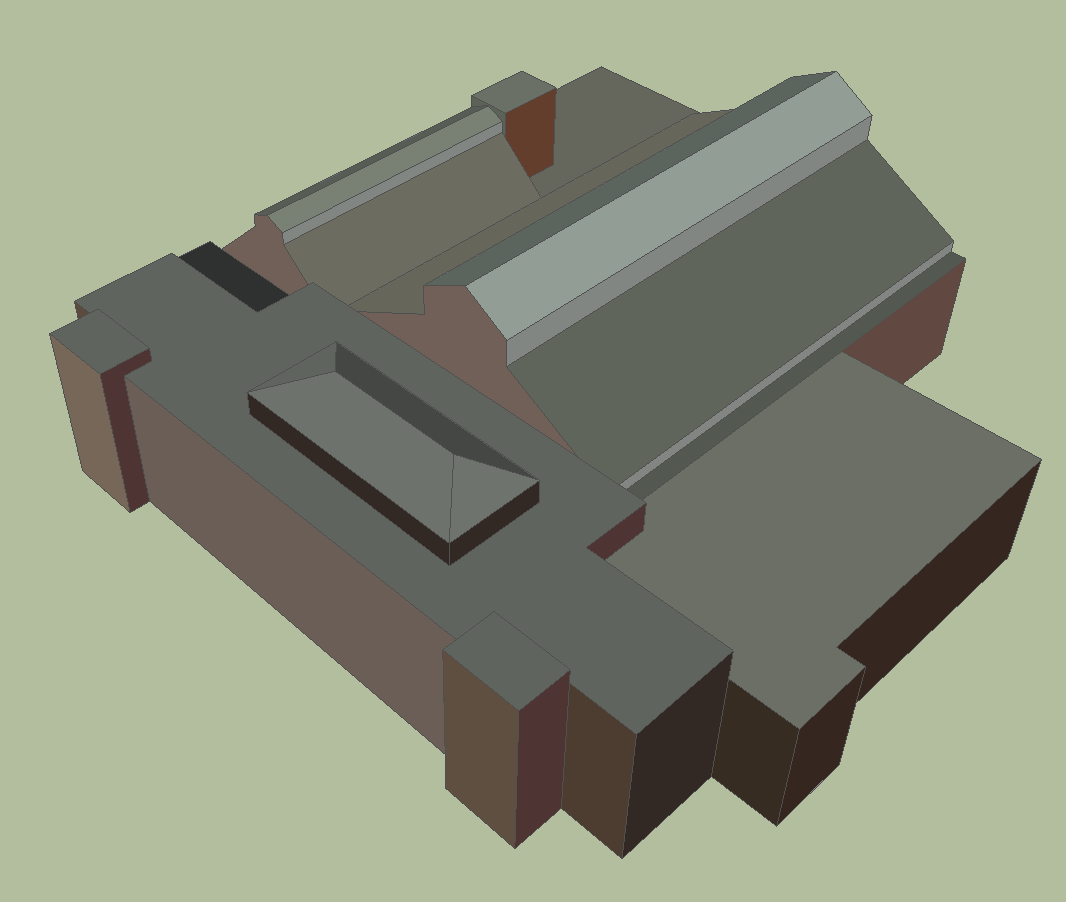
\includegraphics[width=0.5\textwidth]{health_town_1.png} &
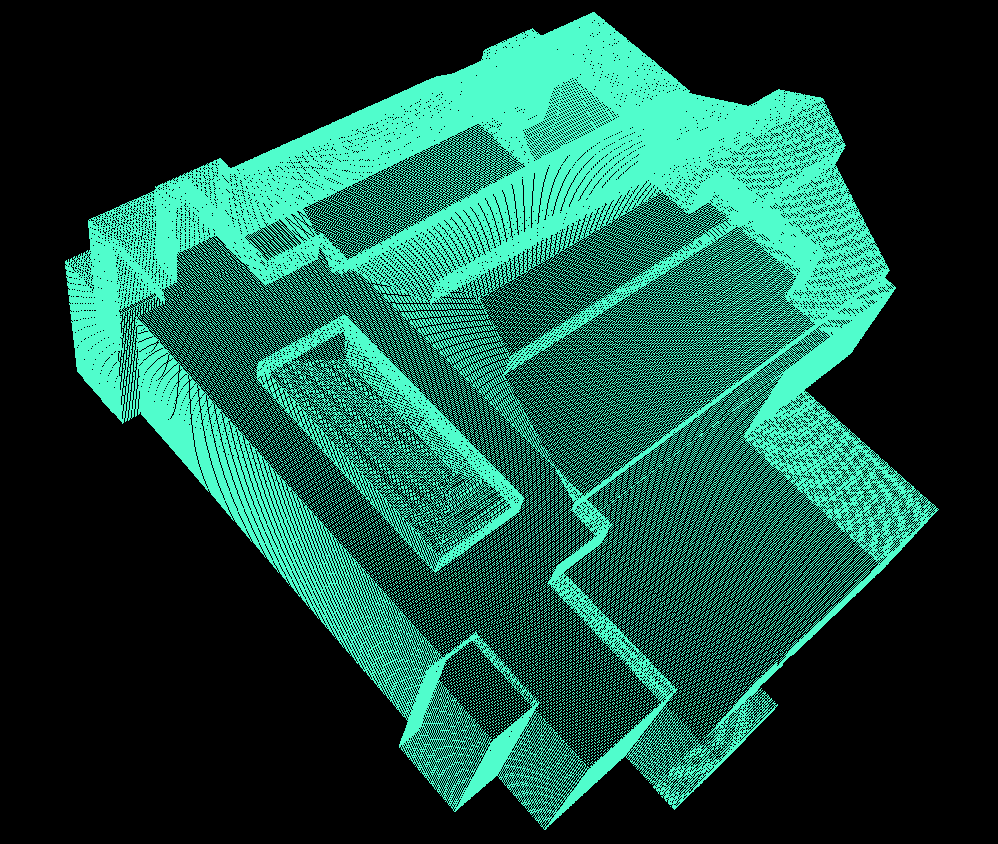
\includegraphics[width=0.5\textwidth]{health_town_2.png} \\
(a) & (b) \\
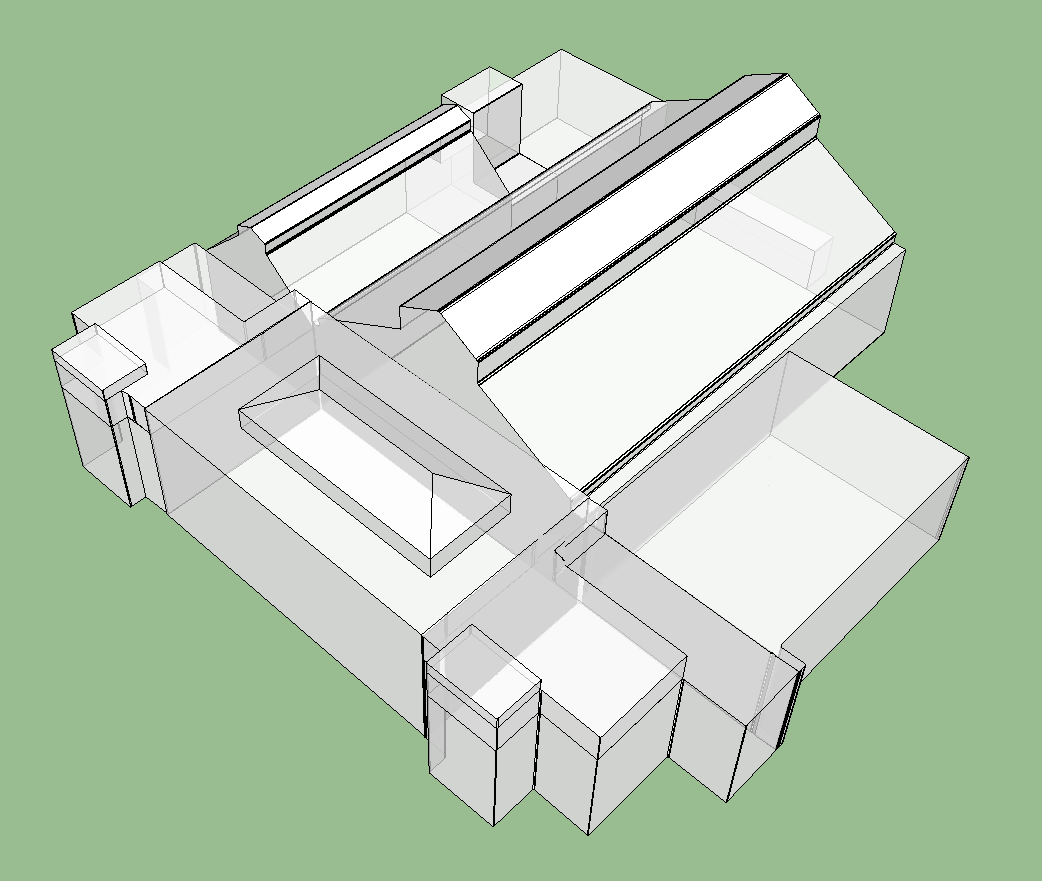
\includegraphics[width=0.5\textwidth]{health_town_3.png} &
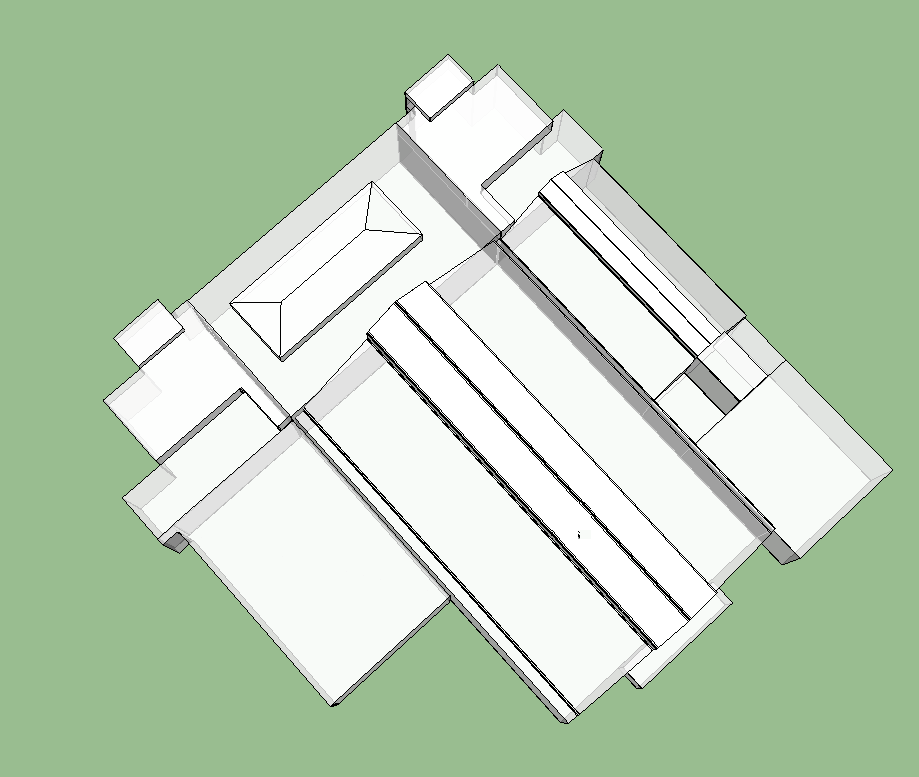
\includegraphics[width=0.5\textwidth]{health_town_4.png} \\
(c) & (d)
\end{tabular}
\end{center}
\caption{Experimental Results of Health Town library model:
      (a) original Sketchup model.
      (b) synthetic point cloud data generated from (a).
      (c) reconstructed model (I) .
      (d) reconstructed model (II).}
\label{fig:ER_Fig7}
\end{figure}

\begin{figure} [htbp]
\begin{center}
\begin{tabular}{cc}
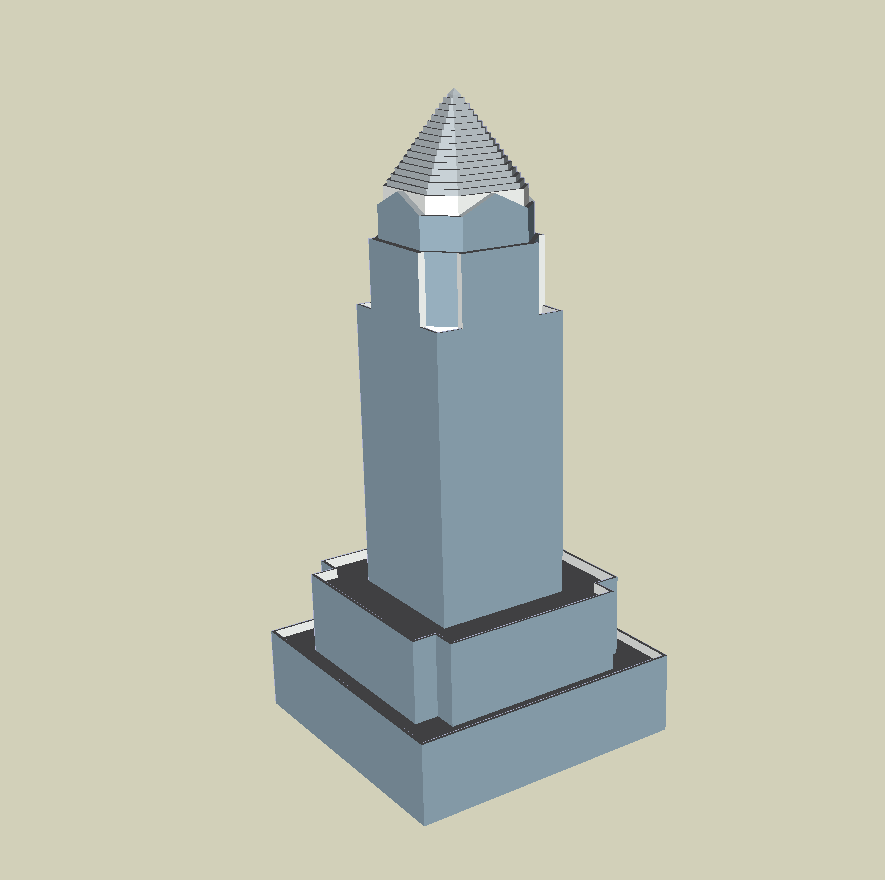
\includegraphics[width=0.5\textwidth]{miami_1.png} &
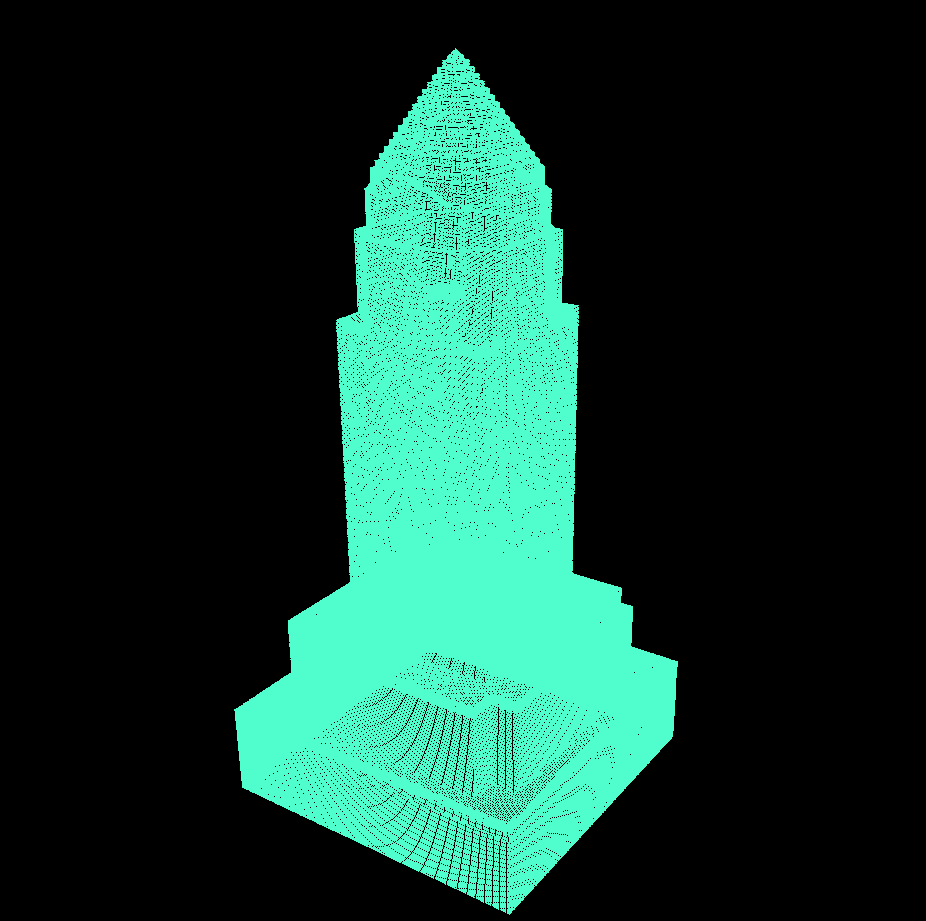
\includegraphics[width=0.5\textwidth]{miami_2.png} \\
(a) & (b) \\
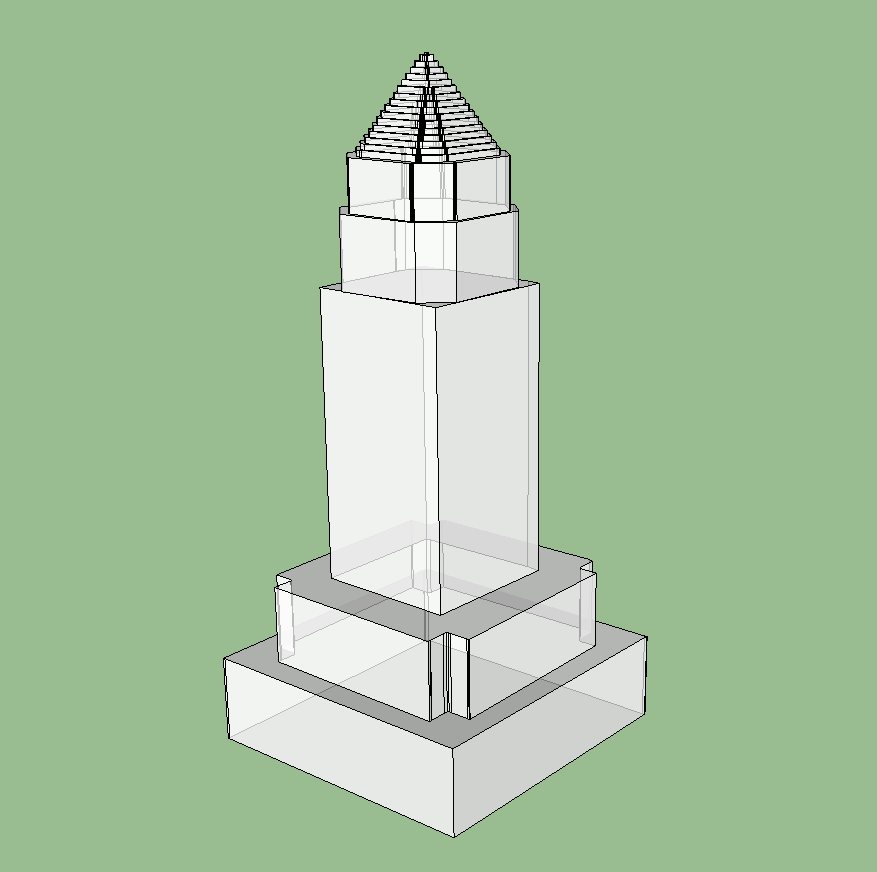
\includegraphics[width=0.5\textwidth]{miami_3.png} &
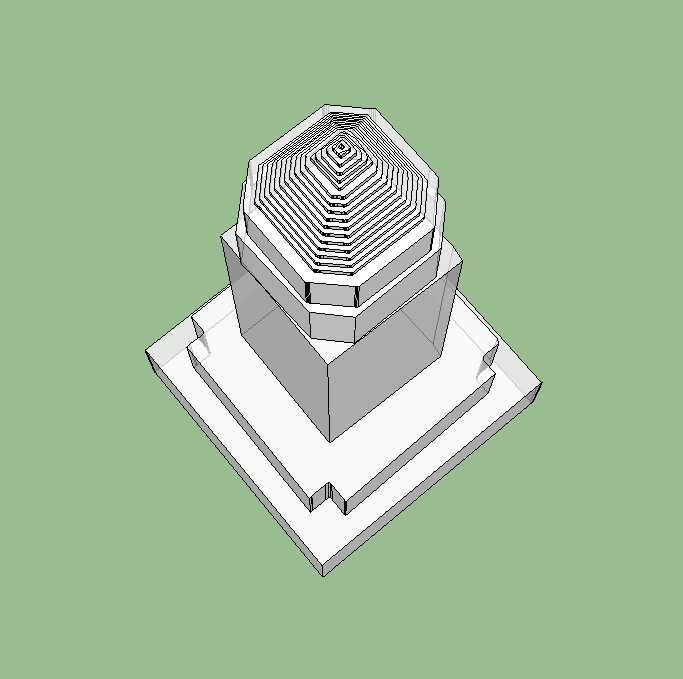
\includegraphics[width=0.5\textwidth]{miami_4.png} \\
(c) & (d)
\end{tabular}
\end{center}
\caption{Experimental Results of Miami Date Court model:
      (a) original Sketchup model.
      (b) synthetic point cloud data generated from (a).
      (c) reconstructed model (I) .
      (d) reconstructed model (II).}
\label{fig:ER_Fig8}
\end{figure}

\begin{figure} [htbp]
\begin{center}
\begin{tabular}{cc}
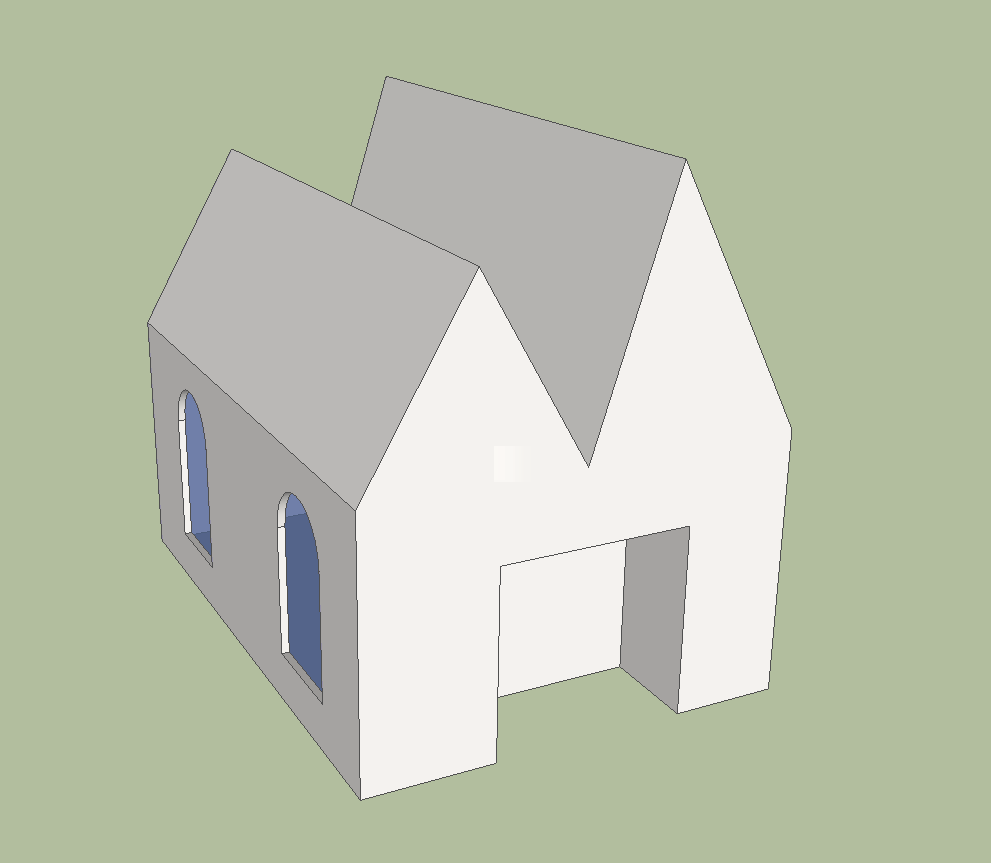
\includegraphics[width=0.5\textwidth]{simple_1.png} &
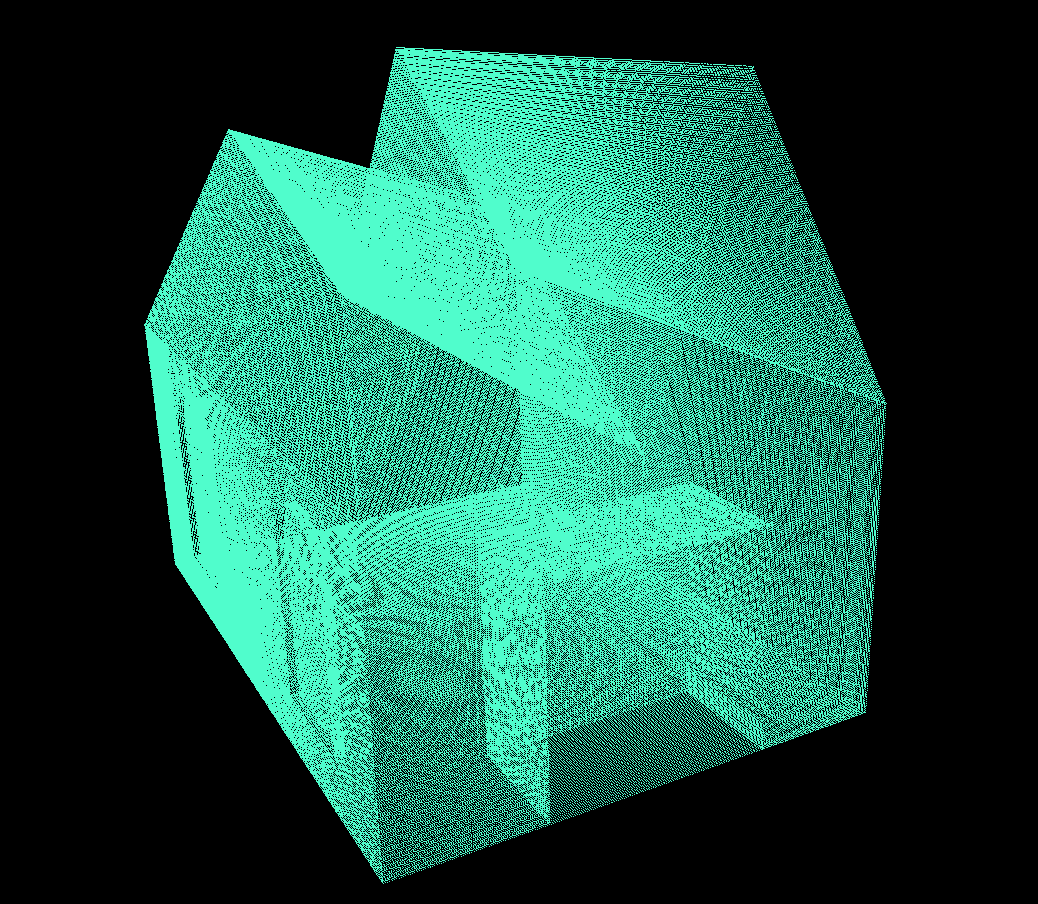
\includegraphics[width=0.5\textwidth]{simple_2.png} \\
(a) & (b) \\
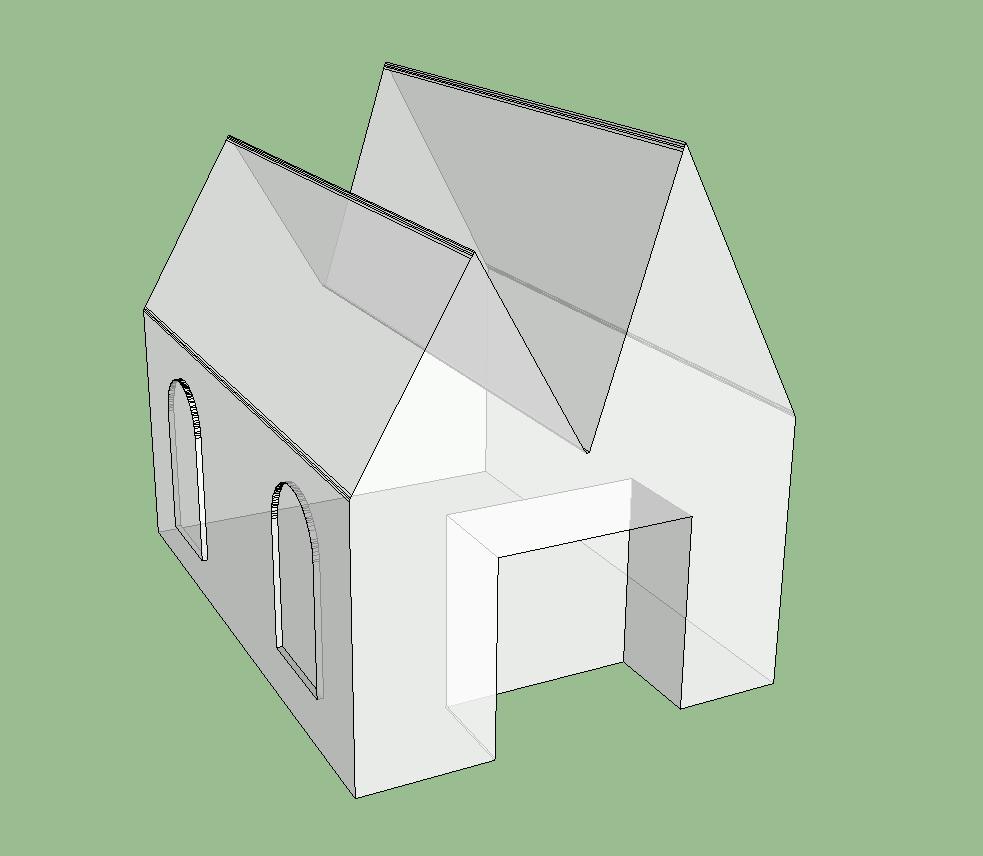
\includegraphics[width=0.5\textwidth]{simple_3.png} &
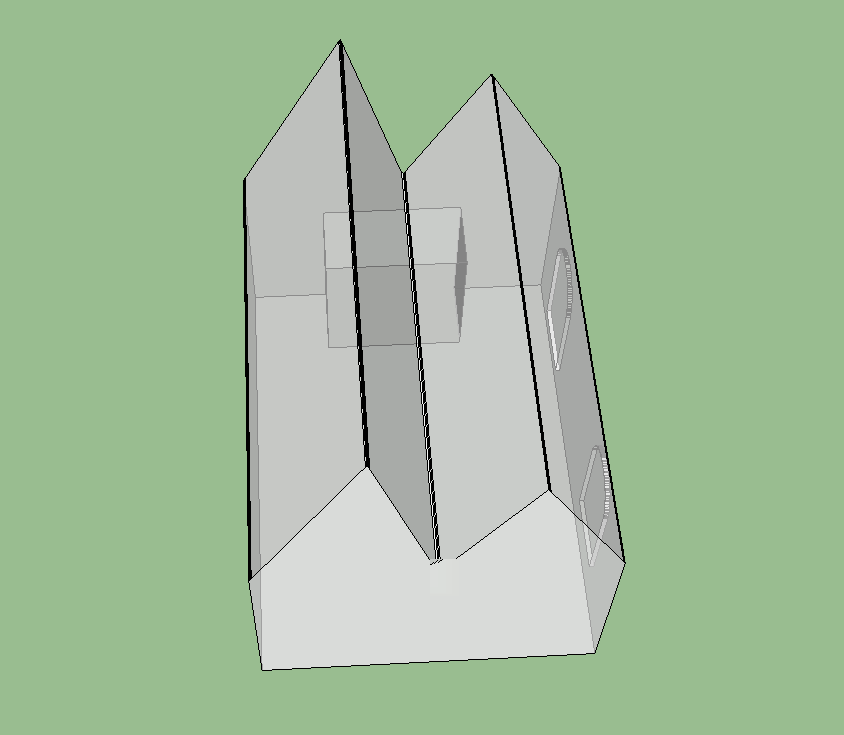
\includegraphics[width=0.5\textwidth]{simple_4.png} \\
(c) & (d)
\end{tabular}
\end{center}
\caption{Experimental Results of simple model:
      (a) original Sketchup model.
      (b) synthetic point cloud data generated from (a).
      (c) reconstructed model (I) .
      (d) reconstructed model (II).}
\label{fig:ER_Fig9}
\end{figure}

\begin{figure} [htbp]
\begin{center}
\begin{tabular}{cc}
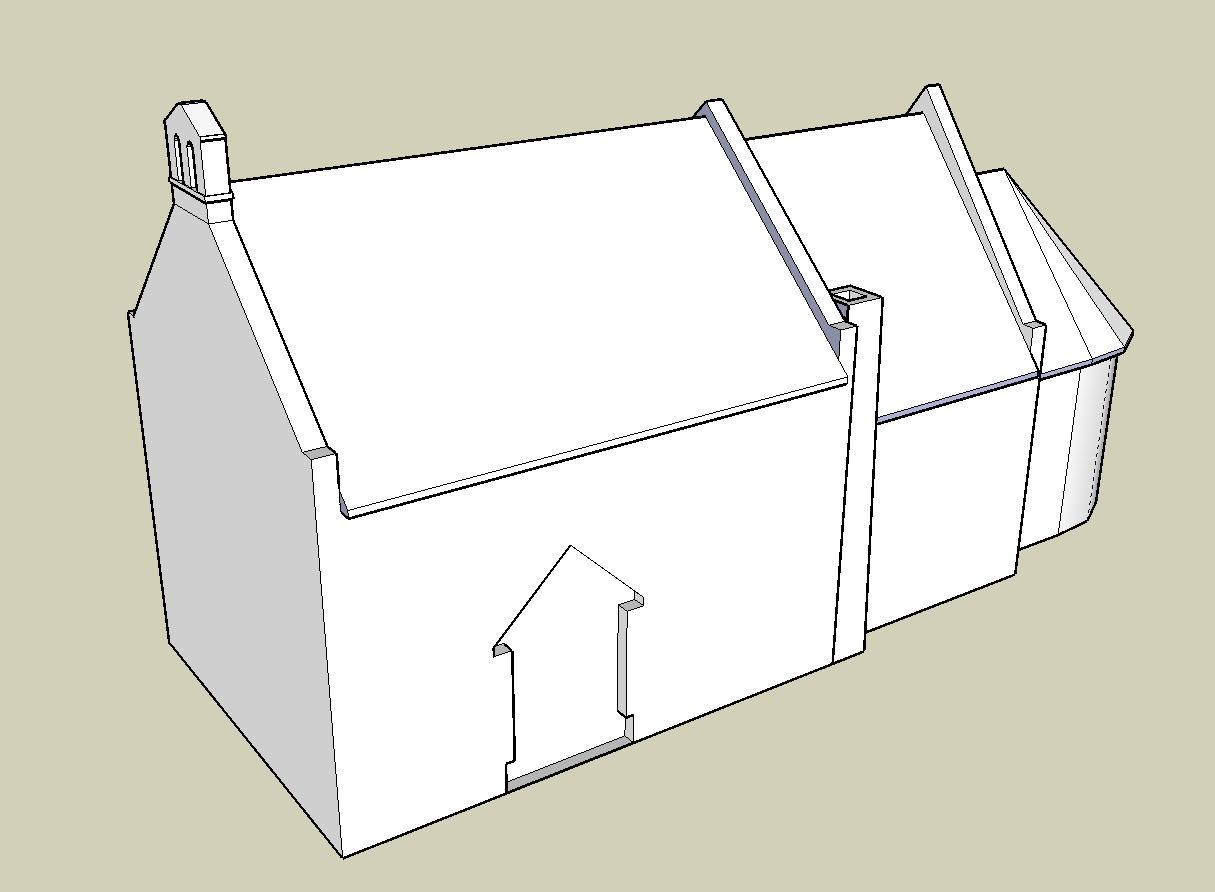
\includegraphics[width=0.5\textwidth]{michael_1.png} &
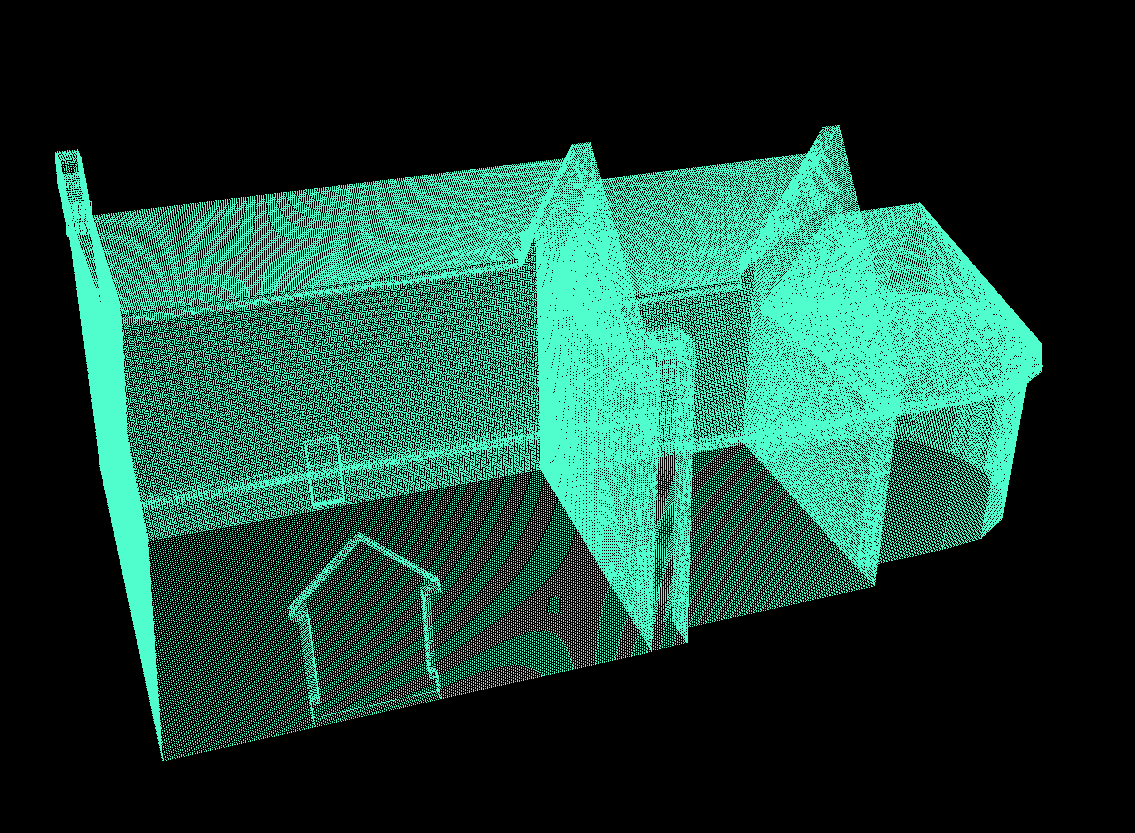
\includegraphics[width=0.5\textwidth]{michael_2.png} \\
(a) & (b) \\
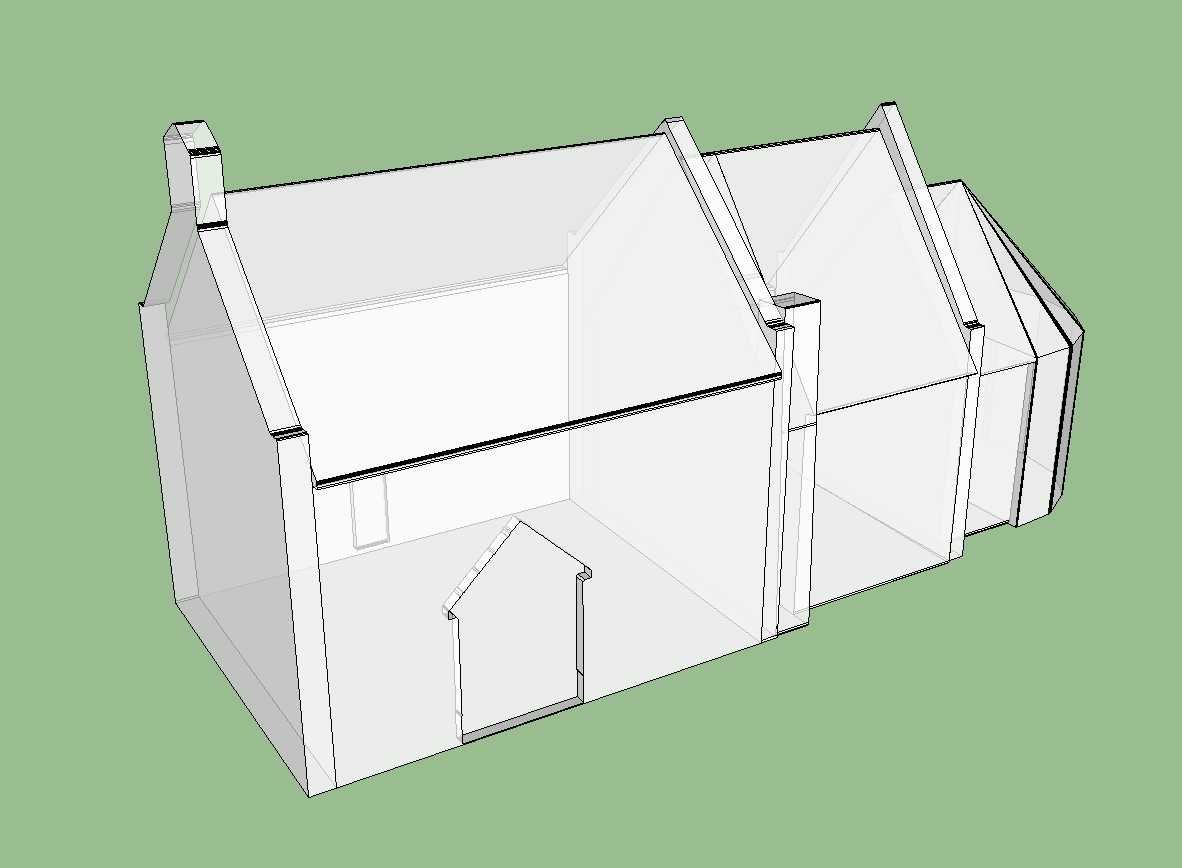
\includegraphics[width=0.5\textwidth]{michael_3.png} &
\includegraphics[width=0.5\textwidth]{michael_4.png} \\
(c) & (d)
\end{tabular}
\end{center}
\caption{Experimental Results of St Michael church model:
      (a) original Sketchup model.
      (b) synthetic point cloud data generated from (a).
      (c) reconstructed model (I) .
      (d) reconstructed model (II).}
\label{fig:ER_Fig10}
\end{figure}

\begin{figure} [htbp]
\begin{center}
\begin{tabular}{cc}
\includegraphics[width=0.5\textwidth]{limitation_1.png} &
\includegraphics[width=0.5\textwidth]{limitation_2.png}
\end{tabular}
\end{center}
\caption{Examples of failed cases:
      (a) intersection of two extruded structures.
      (b) intersection of a taper structure with an extruded structure.}
\label{fig:ER_Lmt}
\end{figure}

%% We need to consider keyslice detection and segmentation.
%%
%% 0. major direction/normal detection. (Hadi's planar HT)
%%
%% 1. exam keyslices from all possible directions, including bottom-up, normals of facades.
%%
%% 2. pick up a direction based on the number of keyslices:
%%
%%   2.1. If there is only one keyslice found in a particular direction, stop.
%%   2.2. If a separator (big trunk data) is detected, mark this slice for segmentation.
%%   2.3. If high frequency keyslices starting from a keyslice $k_i$, mark $k_i$.
%%   2.4. For bottom up direction, segment the data based on 2.2 and 2.3.
%%   2.5. For facade direction, where normals(unit) fall into the same plane, construct an image with inputs of all marked pages.
%%
%% 3. for each segmented point cloud $R_i$, go back to 1.
%%
%% 4. only consider separator as segmentation mark, ignore the extrusion with taper without separator.
%%
%% LIMITATION:
%% *. Could not handle sub-component with extrusion coupled with tapered structure where the separation direction is not
%%    the same as the tapered direction.
%% *. Could not handle intersection of two extrusions from different directions.



% LocalWords:  chapt keyslice fixpoint lr DS keyslices mx WD BPA vertices htbp
% LocalWords:  WDR Sketchup Lmt Spitak pdf CC CCs png downloaded
